\documentclass[11pt, twoside, openright, hidelinks]{book}

%% - - - - - - - - - - - - - - - - - - - - - - - - - - - - - - - - - - - - - %%
%%                               Load Packages                               %%
%% - - - - - - - - - - - - - - - - - - - - - - - - - - - - - - - - - - - - - %%

\usepackage[
  centering,
  head=13.6pt
]{geometry}
\geometry{a4paper}

\usepackage{fontspec}
\directlua{
  luaotfload.add_fallback ("fallbackscript",
  {
    "freeserif:mode=harf;script=dev2;color=000000;",
  })
}

\setmainfont{latinmodernroman}[RawFeature={fallback=fallbackscript}]

\usepackage[italian,main=english]{babel} %% language

\usepackage[a-3u,mathxmp]{pdfx}

\directlua{pdf.setminorversion(5)}

\pagestyle{headings}

\usepackage{scrlayer-scrpage}

\ifoot[]{}
\cfoot[]{}
\ofoot[\pagemark]{\pagemark}
\pagestyle{scrplain}

\usepackage[
  backend=biber,
  style=numeric,
  bibencoding=utf8,
]{biblatex} %% for citations
\addbibresource{document.bib}

\usepackage{import} %% specify path for import

%% math packages
\usepackage{graphicx} %% for pictures
\usepackage{float}
\usepackage{amssymb} %% math symbols
\usepackage{amsmath} %% math matrix etc
\usepackage{minted} %% code block
\usepackage{tabularray} %% better tables
\usepackage{tblr-extras}
\usepackage{booktabs} %% rules for tables
\usepackage{mathrsfs}
\usepackage{mathtools}
\usepackage{algorithm} %% for algorithms
\usepackage{algpseudocode} %% loads algorithmicx
\usepackage{amsthm}
\usepackage{thmtools} %% theorems
\usepackage{simplebnf}
\usepackage{stmaryrd}
\usepackage{ebproof}
\usepackage{xfrac}
%\usepackage{caption}
\usepackage{bytefield}

%% plot packages
\usepackage{pgfplots} %% plots used with \begin{tikzpicture}
\usepackage{tikz} %% for pictures
\pgfplotsset{width=10cm,compat=newest}
\usepackage{subcaption}

%% design packages
\usepackage{enumitem} %% for lists and enumerating
\usepackage{luacolor}
\usepackage{xcolor} % xcolor for defining colors, colortbl for table colors
\usepackage{colortbl} % xcolor for defining colors, colortbl for table colors
\usepackage{makecell} %% for multiple lines in cell of table
\usepackage{cancel}
\usepackage{pgfornament} %% ornaments
\usepackage{makeidx}

%% load last
\usepackage{csquotes} %% correct language also for citations
\usepackage{hyperref} %% links for table of contents, load last
\usepackage{bookmark} %% for better table of contents

%% - - - - - - - - - - - - - - - - - - - - - - - - - - - - - - - - - - - - - %%
%%                       Configuration of the packages                       %%
%% - - - - - - - - - - - - - - - - - - - - - - - - - - - - - - - - - - - - - %%

\linespread{1}
\raggedbottom %% spaces if page is empty % chktex 1

%% set max table of contents recursion to subsection (3->subsubsecition)
\setcounter{tocdepth}{3}
\setcounter{secnumdepth}{3}

%% use bar instead of arrow for vectors
\renewcommand{\vec}[1]{\bar{#1}}
%% easy norm
\newcommand{\norm}[1]{\left\lvert#1\right\rvert}

% argmin and argmax
\DeclareMathOperator*{\argmax}{argmax}
\DeclareMathOperator*{\argmin}{argmin}

%% itemize use less vertical space (use olditemize for default behaviour)
\let\olditemize=\itemize%% old itemize
\let\endolditemize=\enditemize%% old end itemize
\renewenvironment{itemize}{\olditemize\itemsep-0.2em}{\endolditemize}

%% items in itemize emph+box
%% usage: \ieb{Class:} for simple item
%%        \ieb[4cm]{Class:} for specific size of box
\newcommand{\ieb}[2][2cm]{
        \makebox[#1][l]{\emph{#2}}
} %% TODO: replace with description environment (? maybe)

% less vertical space around align & align*
\newcommand{\zerodisplayskips}{
  \setlength{\abovedisplayskip}{0pt}
  \setlength{\belowdisplayskip}{0pt}
  \setlength{\abovedisplayshortskip}{0pt}
  \setlength{\belowdisplayshortskip}{0pt}
}

% make dotfill use all the space available
\renewcommand{\dotfill}{
  \leavevmode\cleaders\hbox to 1.00em{\hss .\hss }\hfill\kern0pt } % chktex 1 chktex 26

\setlength{\fboxsep}{-\fboxrule} % for debugging


%% PACKAGE algorithm
\floatname{algorithm}{Algorithm}


%% PACKAGE tabularray
\UseTblrLibrary{amsmath}
\UseTblrLibrary{caption}
\TblrCaptionBelow%


%% PACKAGE color
\definecolor{red}{rgb}{1, 0.1, 0.1}
\definecolor{lightgreen}{rgb}{0.55, 0.87, 0.47}
\definecolor{gray}{rgb}{0.3, 0.3, 0.3}
\newcommand{\lgt}{\cellcolor{lightgreen}} %% light green in tables
\newcommand{\gry}{\textcolor{gray}} %% gray text
\newcommand{\rd}{\textcolor{red}} %% red text
\newcommand{\green}{\textcolor{green}} %% green text
\newcommand{\blue}{\textcolor{blue}} %% blue text

%% PACKAGE minipage
\newcommand{\thend}[1]{\begin{center}
  \begin{minipage}[c][1em][c]{#1}
    \dotfill{}
  \end{minipage}
\end{center}}


%% PACKAGE thmtools
\declaretheoremstyle[
 headfont=\normalfont\bfseries,
 notefont=\mdseries,
 bodyfont=\normalfont,
 qed=\qedsymbol % chktex 1
]{steo}
\declaretheorem[numbered=yes, style=steo]{theorem}

\declaretheoremstyle[
 headfont=\normalfont\bfseries,
 notefont=\mdseries,
 bodyfont=\normalfont,
 qed=\qedsymbol % chktex 1
]{slem}
\declaretheorem[numbered=yes, style=slem]{lemma}

\declaretheoremstyle[
  headfont=\normalfont\bfseries,
  notefont=\mdseries,
  bodyfont=\normalfont,
]{sdef}
\declaretheorem[numbered=yes, style=sdef]{definition}

\declaretheoremstyle[
  spaceabove=-6pt,
  spacebelow=6pt,
  headfont=\normalfont\bfseries,
  bodyfont=\normalfont,
  postheadspace=1em,
  qed=$\blacksquare$,
  headpunct={:}
]{sprf}
\declaretheorem[name={Proof}, style=sprf, numbered=yes]{prof}

%% ......................................................................... %%
%% local changes
% \setcounter{secnumdepth}{0}
\newcommand{\defeq}{\vcentcolon=}

\usetikzlibrary{trees, positioning, shapes.misc, positioning, arrows.meta}

\DeclarePairedDelimiter\abs{\lvert}{\rvert}%
\DeclarePairedDelimiter\doublesq{\llbracket}{\rrbracket}%


\definecolor{color_Error}{HTML}{FC2836}

\definecolor{color_String}{HTML}{0E7AFF}
\definecolor{color_Path}{HTML}{1AC9D8}
\definecolor{color_Svg}{HTML}{86868B}
\definecolor{color_PositiveInt}{HTML}{1BD5B6}
\definecolor{color_Symbol}{HTML}{5A61FF}

\definecolor{color_System}{HTML}{FECF0A}
\definecolor{color_Environment}{HTML}{FFEDA4}
\definecolor{color_Set}{HTML}{FFE370}
\definecolor{color_Context}{HTML}{D9AF00}
\definecolor{color_Reactions}{HTML}{A78700}

\definecolor{color_Experiment}{HTML}{FD7E25}

\definecolor{color_PositiveSystem}{HTML}{A77753}
\definecolor{color_PositiveEnvironment}{HTML}{F3D2BA}
\definecolor{color_PositiveSet}{HTML}{C99D7D}
\definecolor{color_PositiveContext}{HTML}{875733}
\definecolor{color_PositiveReactions}{HTML}{683A18}

\definecolor{color_Trace}{HTML}{FC577D}
\definecolor{color_PositiveTrace}{HTML}{FB003B}

\definecolor{color_Graph}{HTML}{2ECC46}
\definecolor{color_PositiveGraph}{HTML}{00961A}

\definecolor{color_DisplayNode}{HTML}{B2F4BD}
\definecolor{color_DisplayEdge}{HTML}{81E793}
\definecolor{color_ColorNode}{HTML}{3BC553}
\definecolor{color_ColorEdge}{HTML}{1CB236}

\definecolor{color_AssertFunction}{HTML}{CF00EE}
\definecolor{color_GroupFunction}{HTML}{750086}
\definecolor{color_PositiveAssertFunction}{HTML}{35C9FD}
\definecolor{color_PositiveGroupFunction}{HTML}{02B7F3}


%% - - - - - - - - - - - - - - - - - - - - - - - - - - - - - - - - - - - - - %%

\title{Document}
\author{
  Elvis Rossi
}
\date{\today}

\makeindex

%% - - - - - - - - - - - - - - - - - - - - - - - - - - - - - - - - - - - - - %%

\begin{document}

\pagenumbering{roman}

\begin{titlepage}
  \begin{figure}[!htb]
    \centering
    \includegraphics[keepaspectratio=true,scale=0.5]{figures/cherubino.eps}
  \end{figure}

  \begin{center}
    \LARGE{UNIVERSITY OF PISA}
    \vspace{5mm}
    \\ \Large{Department of Computer Science}
    \vspace{5mm}
    \\ \LARGE{Master Degree in Computer Science}
  \end{center}
  \centering
  \vspace{15mm}
  {\Large{\bf Modeling Reaction Systems}}
  \vspace{40mm}

  \begin{tblr}{colspec={Q[c,l]X[1,m]Q[c,l]}}
    \large{Supervisor:} & & \large{Candidate:} \\
    \textbf{\large{Prof. Roberto Bruni}} & & \textbf{\large{Elvis Rossi}} \\
    \textbf{\large{Prof. Roberta Gori}} \\
    \textbf{\large{Prof. Paolo Milazzo}} \\
  \end{tblr}

  \vspace*{\fill}

  \hrulefill%

  \centering{\large{ACADEMIC YEAR 2025/2026}}

\end{titlepage}


\newpage
\null % chktex 1
\vspace*{\fill}
\begin{center}
  \color{black!30}\pgfornament[width=2cm]{123}
\end{center}
\newpage

\tableofcontents

\newpage
\pagenumbering{arabic}
\setcounter{page}{1}

\begin{chapter}{Introduction}
  Reaction System (RS) is a successful computational framework inspired by biological system,
  first described in\ \cite{Ehrenfeucht_Rozenberg_2004, Ehrenfeucht_Rozenberg_2007}.
  The interaction between biochemical reactions and the functioning of single reactions is based on the mechanisms of facilitation and inhibition.
  Facilitation and inhibition are key concepts in molecular biology\ \cite{Clark_Pazdernik_McGehee_2018}: gene promoters, both in lower and higher organisms, function poorly or not at all in the absence of extra proteins known as gene activator proteins, or transcription factors.
  Other promoters may be inherently active: these are often controlled by a class of gene regulator proteins known as repressors that act to turn genes off.
  Reaction Systems aims to models cell biology by represent this complex interaction between inducers and genes.

  A Reaction System consists of a set of entities and a set of reactions over such entities. Each reaction if enabled produces a set of entities P (called products). A reaction is enabled if its set R (called reactants) is wholly present and if the set I (called inhibitors) of entities is completely absent.
  The use of inhibitors induces non-monotonic behaviors that are difficult to analyze.
  Entities can also be provided by an external context sequence to simulate interaction with an environment, based on a structural operational semantics (SOS) coupled with different transformations and new frameworks aiming at analyzing causal properties that have been developed during the past years\ \cite{Brodo_Bruni_Falaschi_2021, Brodo_Bruni_Falaschi_Gori_Milazzo_Montagna_Pulieri_2024, Brodo_Bruni_Falaschi_Gori_Milazzo_2025}.
  A comprehensive overview of all the different transformations and techniques implemented in the proposed tool are listed in chapter\ \ref{background_chap}.

  Despite the rich theoretical development of Reaction Systems, practical tools for working with RS models have lagged behind. Numerous versions of Prolog and Python programs have been developed\cite{BioResolve2025}, but have problems regarding performance and usability.
  This technological barrier caused by lack of appropriate software may hinder future developments.

  This thesis aims to bridge the gap between the theoretical foundations of Reaction Systems and their practical application. To achieve this a new software platform for modeling, analyzing and designing Reaction Systems is proposed.

  \begin{section}{Software Design and Key Features}
    The core contribution of this work is a new software tool built from the ground up to support Reaction Systems modeling and analysis. Equal emphasis has been placed on performance and user experience. The software is implemented in Rust\cite{rust_2025}, a modern systems programming language chosen for its efficiency and reliability.
    Rust’s strong performance characteristics (memory safety, speed, and concurrency support) help to ensure that even larger Reaction System models can be analyzed quickly, while its emphasis on code safety and clarity makes the tool more maintainable in the long term.

    The platform provides two user interfaces to accommodate different user needs. A command-line interface (CLI) is available for quick integration in already existing pipelines. The CLI allows specification of Reaction Systems and instructions over them and is easily expandable to meet the need of the programmer.

    A graphical user interface (GUI) is also available both as standalone native application and as a static web application running on WebAssembly\cite{WebAssemblyCoreSpecification2}. The GUI lowers the learning curve for new users: instead of writing code or scripts, one can construct reactions, run simulations and view results through the same interface through interactive diagrams and controls. By providing both CLI and graphical native/web interfaces, the tool caters to a wide audience.

    Key capabilities of the developed Reaction Systems software include:

    \begin{itemize}
    \item Graphical interface for modeling and simulation: An interactive GUI that allows users to graphically define RS components and simulate their behavior.
    \item Trace slicing: tools for examining execution traces in detail. Trace slicing allows a user to isolate and inspect specific segments of a reaction sequence, exploring causality between produced elements or inhibited reactions.
    \item Bisimulation analysis: support for formal bisimulation analysis, which enables comparing different Reaction Systems models for behavioral equivalence. The methods are not restricted to just analyzing RS, but are available for any graph-like structure.
    \item Conversion between Reaction Systems and Positive Reactions Systems: to better explore traces and causality, a more suitable model is provided. Conversion between systems is handled automatically and the defaults can be fine tuned or overridden.
    \end{itemize}

    Together, these features make the software a comprehensive environment for working with Reaction Systems. The user can construct, simulate and analyze the results through multiple lenses: from observing cyclic behaviors to checking formal equivalences and visualizing interaction networks.
  \end{section}
\end{chapter}

\begin{chapter}{Background}\label{background_chap}
  \begin{section}{Reaction Systems}
    Reaction Systems are a qualitative model inspired by biochemical processes.
    The behavior is described by reactions, each of them requiring some reactants \(R\) and requiring the absence of inhibitors \(I\) to produce some product elements \(P\). ``Elements'' and ``entities'' will be used interchangeably to refer to elements of these sets.

    \begin{definition}[Reaction]
      A reaction is a triplet a \(= (R, I, P)\), where \(R, I, P\) are finite sets with \(R \cap I = \emptyset\) and \(R, I, P \neq \emptyset\). If \(S\) is a set such that \(R, I, P \subseteq S\), then a is a reaction in \(S\).
    \end{definition}

    The reactions \((R, I, P)\) operate over a finite set of entities \(S\), called \textit{background set}.
    The theory of RSs is based on three assumptions:
    \begin{itemize}
    \item\label{first_assumption} no permanency, meaning entities vanish unless sustained by a reaction;
    \item\label{second_assumption} no counting, meaning the exact quantity of each entity is irrelevant;
    \item threshold nature of resources, meaning if an entity is present, it is present for all possible reactions.
    \end{itemize}

    \begin{definition}
      Let \(T\) be a finite set.
      \begin{enumerate}
      \item Let \(a\) be a reaction. Then \(a\) is enabled by \(T\), denoted by \(en_{a}(T)\) if \(R_a \subseteq T\) and \(I_a \cap T = \emptyset\). The result of \(a\) on \(T\), denoted by \(res_{a}(T)\), is defined by: \(res_{a}(T) \defeq P_a\) if \(en_a(T)\) and  \(res_{a}(T) \defeq \emptyset\) otherwise.
      \item Let \(A\) be a finite set of reactions. The result of \(A\) on \(T\), denoted by \(res_A(T)\), is defined as \(res_A(T) \defeq \bigcup_{a \in A}{res_{a}(T)} \).
      \end{enumerate}
    \end{definition}

    Note that by virtue of the second assumption \hyperref[second_assumption]{(2)} if two reactions \(a, b \in A\), with both \(a\) and \(b\) enabled by T, then even if \(R_a \cap R_b \neq \emptyset\), still both \(P_a \subseteq res_A(T)\) and \(P_b \subseteq res_A(T)\). Both reactions can use \(R_a \cap R_b\) to produce their products.
    This would not be allowed in other models such as Petri nets\ \cite{Rozenberg_Engelfriet_1998}, a common model of concurrent systems.

    Let \(rac(S)\) be the set of all the reactions in \(S\).

    \begin{definition}[Reaction System]
      A Reaction System (RS) is a pair \(\mathcal{A} = (S, A)\) such that \(S\) is a finite set and \(A \subseteq rac(S)\) is a finite set of reactions in S.
    \end{definition}

    The set \(S\) is called the \textit{background set} of \(\mathcal{A}\); its elements, called \textit{entities}, represent molecular entities (e.g.\ atoms, ions, molecules) that may be present in the state of the system modeled by \(\mathcal{A}\). The set \(A\) is called the \textit{set of reactions} of \(\mathcal{A}\). Since \(S\) is finite, so is \(A\).

    the behavior of a RS is formalized through the notion of an interactive process.

    \begin{definition}[Interactive Process]
      Let \(\mathcal{A} = (S, A)\) be a RS and let \(n > 0\). An \(n\)-step interactive process in \(\mathcal{A}\) is a pair \(\pi = (\gamma, \delta)\) such that \(\gamma \defeq {\left\{C_i\right\}}_{i\in [0, n]}\) is the context sequence and \(\delta \defeq {\left\{D_i\right\}}_{i\in [0, n]}\) is the result sequence, where \(\forall i \in [0, n], C_i, D_i \subseteq S\), \(D_0 = \emptyset\) and \(\forall i \in [0, n-1], D_{i+1} \defeq res_A(D_i \cup C_i)\).
      We call \(\tau \defeq W_0, \ldots, W_n\) the state sequence, where \(W_i \defeq C_i \cup D_i\) for all \(i \in [0, n]\).
    \end{definition}

    \begin{figure}[h]
      \def\svgwidth{\linewidth}
      \import{figures}{reaction_system.pdf_tex}
      \caption{Interactive process of a reaction system.}
    \end{figure}

    Note that \(C_i\) and \(D_i\) do not have to be disjointed.

    \(W_0 = C_0\) is called the initial state of \(\pi\). If \(C_i \subseteq D_i\) for all \(i \in [1, n]\) then \(\pi\) is called context-independent. For context-independent interactive process, we can take \(C_i = \emptyset\) for all \(i = [1, n]\) without changing the state sequence.

    In a context-independent state sequence \(\tau = W_0, \ldots, W_i, W_{i+1}, \ldots, W_n \), during the transition from \(W_i\) to \(W_{i+1}\) all entities from \(W_i -res_{\mathcal{A}}(W_i)\) will not persist. This reflects the assumption of no permanency \hyperref[first_assumption]{(1)}. Thus, if \(\tau\) is not context-independent, an entity from a current state can also be sustained by the context \(C_{i+1}\).

    \begin{definition}[Sequence Shift]
      Let \(\gamma = {\left\{C_i\right\}}_{i\in [0, n]}\) a context sequence. Given a positive integer \(k \leq n\), let \(\gamma^{k} \defeq {\left\{C_{i+k}\right\}}_{i\in [0, n-k]}\).
    \end{definition}

    \begin{subsection}{Example: A binary counter}\label{binary_counter}
      A reaction system can act as a cyclic n-bit counter in which external signals trigger increment or decrement operations. To build the counter, let \(n > 0\) be an integer and define the background set as \( \{p_0, p_1, \ldots, p_{n-1}\} \cup \{ dec, inc\} \).

      Five sets of reactions describe a binary counter-like behavior:

      % \begin{center}
      %   \begin{tblr}{colspec={Q[l,m]Q[l,m]Q[l,m]}, colsep=2pt}
      %     \(a_j\) &= \((\{p_j\}, \{dec, inc\}, \{p_j\})\), &\(\forall j \in [0, n]\)\\
      %     \(b_j\) &= \((\{inc, p_0, p_1, \ldots, p_{j-1}\}, \{dec, p_j\}, \{p_j\})\), &\(\forall j \in [0, n]\)\\
      %     \(c_{j,k}\) &= \((\{inc, p_k\}, \{dec, p_j\}, \{p_k\})\), &\(\forall j, k \text{s.t.} 0 \leq j < k < n\)\\
      %     \(d_j\) &= \((\{dec\}, \{inc, p_0, p_1, \ldots, p_j\}, \{p_j\})\), &\(\forall j \in [0, n]\)\\
      %     \(e_{j,k}\) &= \((\{dec, p_j, p_k\}, \{inc\}, \{p_k\})\), &\(\forall j, k \text{s.t.} 0 \leq j < k < n\)\\
      %   \end{tblr}
      % \end{center}

      \begin{center}
        \begin{tblr}{colspec={Q[l,m]Q[l,m]Q[r,m]Q[c,m]Q[l,m]Q[l,m]}, colsep=2pt}
          \(a_j\) &= & \((\{p_j\}, \)& \(\{dec, inc\}, \)& \(\{p_j\})\), &\(\forall j \in [0, n]\)\\
          \(b_j\) &= & \((\{inc, p_0, p_1, \ldots, p_{j-1}\}, \)& \(\{dec, p_j\}, \)& \(\{p_j\})\), &\(\forall j \in [0, n]\)\\
          \(c_{j,k}\) &= & \((\{inc, p_k\}, \)& \(\{dec, p_j\}, \)& \(\{p_k\})\), &\(\forall j, k \text{ s.t. } 0 \leq j < k < n\)\\
          \(d_j\) &= & \((\{dec\}, \)& \(\{inc, p_0, p_1, \ldots, p_j\}, \)& \(\{p_j\})\), &\(\forall j \in [0, n]\)\\
          \(e_{j,k}\) &= & \((\{dec, p_j, p_k\}, \)& \(\{inc\}, \)& \(\{p_k\})\), &\(\forall j, k \text{ s.t. } 0 \leq j < k < n\)\\
        \end{tblr}
      \end{center}


      where reactions \(a\) cause the bits to be restrained in the next state if there is no operation, reactions \(b\) implement the increment operation by flipping the least significant zero to one, reactions \(c\) let the more significant bits remain, reactions \(d\) implements the decrement operation by flipping to one the bits when there is no one at a lower position, and reactions \(e\) let the more significant bits remain.

      The complete RS \(\mathcal{B}_n\) is defined as follows: \(\mathcal{B}_n = \left(S_n, B_n\right)\) where\[S_n = \{p_0, p_1, \ldots, p_{n-1}\} \cup \{dec, inc\}\] and \[B_n = \{a_j, b_j, d_j | 0 \leq k < n\} \cup \{c_{j, k}, e_{j, k} | 0 \leq l < k < n\}\]

      To illustrate the system in action consider the sequence of contexts:
      \(C_0 = \{p1, p3\},\\C_1 = \emptyset, C_2 = \{inc\}, C_3 = \{inc\}, C_4 = \{dec\}, C_5 = \{dec, inc\}\). This gives the result sequence \(\delta = \emptyset.\{p1, p3\}.\{p1, p3\}.\{p0, p1, p3\}.\{p2, p3\}.\{p0, p1, p3\}.\emptyset\) and state sequence\\\(\tau = \{p1, p3\}.\{p1, p3\}.\{p1, p3, inc\}.\{p0, p1, p3, inc\}.\{p2, p3, dec\}.\{p0, p1, p3, dec, inc\}.\emptyset\),\\in binary representation is \(\{1010_2\}.\{1010_2\}.\{1010_2\}.\{1011_2\}.\{1100_2\}.\{1011_2\}.\{0000_2\}\) by ignoring \(inc\) and \(dec\).
    \end{subsection}

    \begin{subsection}{Simple loops}
      The result sequence of a RS, generated by applying the reactions, can be different from \(\emptyset\) for an infinite number of results. But if two results are the same, also the following result will be the same. This implies the existence of a loop of states. To identify a loop one can simply truncate the trace at position \(n\) and search for the result in position \(n+1\) in the truncated trace.

      If the entities provided by the context are not constant, the behavior might not be as easily described. By restricting only on a constant set provided by the context, we can be sure that the computation will find a loop.

      These loops are called \textit{lollipops}.

      For example by providing the set \(\{inc\}\) as the context at each step of the system from Example\ \ref{binary_counter}, we obtain the loop: \(\{p1, p3\}.\{p0, p1, p3\}.\{p2, p3\}.\{p0, p2, p3\}.\{p1, p2, p3\}.\\\{p0, p1, p2, p3\}.\{\}.\{p0\}.\{p1\}.\{p0, p1\}.\{p2\}.\{p0, p2\}.\{p1, p2\}.\{p0, p1, p2\}.\{p3\}.\{p0, p3\}\).
    \end{subsection}
  \end{section}

  \begin{section}{SOS rules for reaction systems}\label{SOS_rules_section}
    The behavior of a RS could be defined as a discrete time interactive process: a finite context sequence describes the entities provided by the environment at each step, the current state is determined by the union of the entities coming from the environment with those produced from the previous step and the state sequence is determined by applying all and only the enabled reactions to the set of entities available in the current state.

    Given the context sequence, the semantics of RSs is uniquely determined and can be represented as a finite, deterministic and labeled or unlabeled transition system.
    RS have had defined a Labeled Transition System (LTS) semantics as seen in\cite{Brodo_Bruni_Falaschi_2021}.

    \begin{definition}[RS processes]
      Let \(S\) be a set of entities. An RS process \(P\) is any term defined by the following grammar:

      \begin{bnf}(relation-sym-map = % chktex 36
        {
          {::=} = {\ensuremath{\Coloneqq}},
          {->} = {},
          {:in:} = {\ensuremath{\subseteq}},
        },)
        $P$ : ::= % chktex 26
        | [$M$] : mixture process % chktex 26
        ;; % chktex 26
        $M$ : ::= % chktex 26
        | $(R, I, P)$ : reaction % chktex 26
        | $D$ : set of entities % chktex 26
        | $K$ : context process % chktex 26
        | $M \vert M$ : parallel composition % chktex 26
        ;; % chktex 26
        $K$ : ::= % chktex 26
        | \textbf{$0$} : nil context % chktex 26
        | $X$ : process variable % chktex 26
        | $C.X$ : {set of entities\\followed by context} % chktex 26
        | $K + K$ : non deterministic choice % chktex 26
        | $\texttt{rec} X . K$ : recursive operator % chktex 26
        ;; % chktex 26
        Where \\ & \(R, I, P\) :in: \(S\) non empty sets of entities : % chktex 26
        ;; % chktex 26
        \(C, D\) :in: \(S\) possibly empty set of entities : % chktex 26
        ;; % chktex 26
        \(X\) -> a process variable : % chktex 26
      \end{bnf}
    \end{definition}

    An RS process \(P\) embeds a mixture process \(M\) obtained as he parallel composition of some reactions \((R, I, P)\), some set of currently present entities \(D\) (possibly the empty set \(\emptyset\)), and some context process \(K\). For brevity sake \(M_1 \vert M_2 \vert M_3 = \prod_{i \in \{1, 2, 3\}} M_i \).
    A process context \(K\) is a possibly nondeterministic and recursive system: the nil context \(\textbf{0}\) stops the computation; the prefixed context \(C.K\) provides the entities in \(C\) and then uses \(K\) as the next context; the non deterministic choice \(K_1 + K_2\) allows the context to behave either as \(K_1\) or \(K_2\); X is a process variable; and \(\texttt{rec} X. K\) is the recursive operator of process algebras. For brevity sake \(K_1 + K_2 + K_3 = \sum_{i \in \{1, 2, 3\}}K_i\).

    \begin{definition}[RSs as RS processes]
      Let \(\mathcal{A}=(S, A)\) be a RS, and \(\pi = (\gamma, \delta)\) an \(n\)-step interactive process in \(\mathcal{A}\) with \(\gamma = {\{C_i\}}_{i \in [0, n]}\) and \(\delta = {\{D_i\}}_{i \in [0, n]}\). For any step \(i \in [0, n]\), the corresponding RS process \(\doublesq{\mathcal{A}, \pi}_i\) is defined as follows:

      \[ \doublesq{\mathcal{A}, \pi}_i \defeq \left[ \prod_{a \in A} a \vert D_i \vert K_{\gamma^i} \right] \]

      where the context process \(K_{\gamma^i} \defeq C_i . C_{i+1}. \ldots . C_n . \textbf{0} \) is the sequentialization of the entities offered by \(\gamma^i\).%% \ \(\doublesq{\mathcal{A}, \pi} = \doublesq{\mathcal{A}, \pi}_0\).
    \end{definition}

    \begin{definition}[Label]
      A label is a tuple \(\langle W \triangleright R, I, P \rangle\) with \( W, R, I, P \subseteq S\).
    \end{definition}
    In a transition label \(\langle W \triangleright R, I, P \rangle\), \(W\) records the set of entities currently in the system (produced in the previous step or provided by the context), \(R\) records the set of entities whose presence is assumed (either because they are needed as reactants on an applied reaction or because their presence prevents the application of some reaction), \(I\) records the set of entities whose absence is assumed, and \(P\) records the set of entities produced by the applied reactions.

    \begin{definition}[Operational Semantics]
      The operational semantics of processes is defined by the set of SOS inference rules in figure\ \ref{SOS_semantics}.
    \end{definition}

    \begin{figure}[!h]
      \centering
      \begin{prooftree}
        \hypo{ \vphantom{K \left[ \sfrac{ \texttt{rec} X.K }{ X } \right] \xrightarrow{\langle W \triangleright R, I, P \rangle} K'} } % chktex 1
        \infer1[(Ent)]{D \xrightarrow{\langle D\ \triangleright\ \emptyset, \emptyset, \emptyset \rangle} \emptyset} % chktex 1
      \end{prooftree}\hspace{1em}
      \begin{prooftree}
        \hypo{ \vphantom{K \left[ \sfrac{ \texttt{rec} X.K }{ X } \right] \xrightarrow{\langle W \triangleright R, I, P \rangle} K'} } % chktex 1
        \infer1[(Ctx)]{C.K \xrightarrow{ \langle C\ \triangleright\ \emptyset, \emptyset, \emptyset \rangle } K} % chktex 1
      \end{prooftree}\hspace{1em}
      \begin{prooftree}
        \hypo{ K \left[ \sfrac{ \texttt{rec} X.K }{ X } \right] \xrightarrow{\langle W \triangleright R, I, P \rangle} K' } % chktex 1
        \infer1[(Rec)]{ \texttt{rec} X.K \xrightarrow{\langle W\ \triangleright\ R, I, P \rangle} K' } % chktex 1
      \end{prooftree}\vspace{2em}

      \begin{prooftree}
        \hypo{ K_1 \xrightarrow{\langle W \triangleright R, I, P \rangle} K_1' } % chktex 1
        \infer1[(Suml)]{ K_1 + K_2 \xrightarrow{\langle W\ \triangleright\ R, I, P \rangle} K_1' } % chktex 1
      \end{prooftree}\hspace{1em}
      \begin{prooftree}
        \hypo{ K_2 \xrightarrow{\langle W \triangleright R, I, P \rangle} K_2' } % chktex 1
        \infer1[(Sumr)]{ K_1 + K_2 \xrightarrow{\langle W\ \triangleright\ R, I, P \rangle} K_2' } % chktex 1
      \end{prooftree}\vspace{2em}

      \begin{prooftree}
        \hypo{ \vphantom{J \cup Q \neq \emptyset} } % chktex 1
        \infer1[(Pro)]{ (R, I, P) \xrightarrow{\langle \emptyset\ \triangleright\ R, I, P \rangle} (R, I, P) \vert P } % chktex 1
      \end{prooftree}\hspace{1em}
      \begin{prooftree}
        \hypo{ J \subseteq I } % chktex 1
        \hypo{ Q \subseteq R } % chktex 1
        \hypo{ J \cup Q \neq \emptyset } % chktex 1
        \infer3[(Inh)]{ (R, I, P) \xrightarrow{\langle \emptyset\ \triangleright\ R, I, P \rangle} (R, I, P) \vert P } % chktex 1
      \end{prooftree}\vspace{2em}

      \begin{prooftree}
        \hypo{ M_1 \xrightarrow{\langle W_1 \triangleright R_1, I_1, P_1 \rangle} M_1' } % chktex 1
        \hypo{ M_2 \xrightarrow{\langle W_2 \triangleright R_2, I_2, P_2 \rangle} M_2' } % chktex 1
        \hypo{ (W_1 \cup W_2 \cup R_1 \cup R_2) \cap (I_1 \cup I_2) } % chktex 1
        \infer3[(Par)]{ M_1 \vert M_2 \xrightarrow{\langle W_1 \cup W_2\ \triangleright\ R_1 \cup R_2, I_1 \cup I_2, P_1 \cup P_2 \rangle} M_1' \vert M_2' } % chktex 1
      \end{prooftree}\vspace{2em}

      \begin{prooftree}
        \hypo{ M \xrightarrow{\langle W \triangleright R, I, P \rangle} M' } % chktex 1
        \hypo{ R \subseteq W } % chktex 1
        \infer2[(Sys)]{ [M] \xrightarrow{\langle W\ \triangleright\ R, I, P \rangle} [M'] } % chktex 1
      \end{prooftree}

      \caption{SOS semantics of the reaction system process}\label{SOS_semantics}
    \end{figure}

    \(K \left[ \sfrac{ \texttt{rec} X.K }{ X } \right]\) denotes the process obtained by replacing in \(K\) every free occurrence of the variable \(X\) with its recursive definition \(\texttt{rec} X.K\).
    The rule (Pro), executes the reaction \((R, I, P)\) (its reactants, inhibitors, and products are recorded the label), which remains available at the next step together with \(P\).
    The rule (Inh) applies when the reaction \((R, I, P)\) should not be executed; it records in the label the possible causes for which the reaction is disabled: possibly some inhibiting entities \((J \subseteq I)\) are present or some reactants \((Q \subseteq R)\) are missing, with \(J \cup Q \neq \emptyset\), as at least one cause is needed for explaining why the reaction is not enabled.
  \end{section}


  \begin{section}{Positive Reaction Systems}
    A particular kind of Reaction Systems, first seen in\ \cite{Brodo_Bruni_Falaschi_Gori_Milazzo_Montagna_Pulieri_2024}, are those without inhibitors. Such reactions are called positive and can be simply written as pairs \((R, P)\) and are equivalent to \((R, \emptyset, P)\). One can always encode any standard RS \(\mathcal{A} = (S, A)\) into an equivalent one without inhibitors. In order to track the absence of entities, a new ``negative'' entity is added for each original one. In any meaningful state \(W = D \cup C\) there will always be either one between \(a\) and \(\bar{a}\), but never both. As a consequence, for any entity \(a \in S_C\), we must assume that the context will provide either \(a\) or \(\bar{a}\).
    Define \(\textbf{S} \defeq S \uplus \bar{S} \) and \( \bar{S} \defeq \{ \bar{a} \vert a \in S\}\). A subscript \(D\) or \(C\) will be used to differentiate between entities related to reaction products and related to the context.

    \begin{definition}[State consistency]
      A set \(\textbf{W} \subseteq \textbf{S}\) is non-contradictory if for all entities \(a \in S\) it holds that \(\{a, \bar{a}\} \nsubseteq \textbf{W}\). A non-contradictory state \(\textbf{W} \subseteq \textbf{S}\) is consistent if, for any entity \(a \in S\), either \(a \in \textbf{W}\) or \(\bar{a} \in \textbf{W}\) holds.
    \end{definition}


    \begin{definition}[Positive RS\cite{Brodo_Bruni_Falaschi_Gori_Milazzo_2025}]\label{positive_rs}
      A Positive RS is a Reaction System \(\mathcal{A}^+ = (\textbf{S}, A)\) that satisfies the following conditions:
      \begin{enumerate}
      \item Each reaction \(r\) in \(A\) is positive, i.e., \(r = (\textbf{R}, \emptyset, \textbf{P})\) for some non-contradictory sets \(\textbf{R}\) and \(\textbf{P}\).
      \item Consistency preservation: for any consistent state \(\textbf{W}\), the result set \(res_{\mathcal{A}^+}(\textbf{W})\) must be consistent.\label{second_condition_positive}
      \end{enumerate}
    \end{definition}

    If one assumes that the initial state \(\textbf{D}_0 \subseteq \textbf{S}_D\) is a non-contradictory set and that the sets \(\textbf{C}_0, \ldots, \textbf{C}_n \subseteq \textbf{S}_C\) provided by the context are non-contradictory sets, the second condition of\ \ref{second_condition_positive} guarantees that all result states traversed by the computation will be consistent as well.

    \begin{subsection}{From RSs to Positive RSs}
      For each standard RS \(\mathcal{A} = (S, A)\) it is possible to construct a Positive RS \(\mathcal{A}^+ = (\textbf{S}, A^+)\) that exactly mimic the behavior of \(\mathcal{A}\).
      The reactions in \(A^+\) can be split in two categories: \(A^+_{pos}\) that simply embeds the original reactions \(A\) and \(A^+_{neg}\) whose reactions serve for negative entities bookkeeping.

      For each reaction \((R, I, P) \in A\) there will be one positive reaction \((R \cup \bar{I}, P) \in A^+_{pos}\). Extra reactions are needed to track the absence of the products of the original reactions. They will be produced whenever no reaction in \(A\) that produces \(a\) is enabled. For this purpose, assume to collect all reactions in \(A\) that are capable of producing \(a\): to ensure that none of them are enabled, we must make sure that, for each one, at least one reactant is absent or at least one inhibitor is present.

      \begin{definition}[Prohibiting set]
        Let \(\mathcal{A} = (S, A)\) be RS and \(a \in S_D\) one of its entities. A non-contradictory set \(\textbf{T} \subseteq \textbf{S}\) is a prohibiting set for \(a\) if for any reaction \((R, I, P \cup {a}) \in A\) we have that \(\textbf{T} \cap (I \cup \bar{R}) \neq \emptyset\).
        Denote the set of prohibiting sets for \(a\) with \(\mathit{Proh}_{\mathcal{A}}(a)\).
      \end{definition}

      \begin{definition}[Encoding RSs into PRSs]
        Let \(\mathcal{A} = (S, A)\) be a RS, its encoding into a Positive RS is obtained by considering \(\mathcal{A}^+ \defeq (\textbf{S}, A^+)\) whose set of positive reactions \(A^+ \defeq A^+_{pos} \cup A^+_{neg}\) is defined as follows:
        \begin{align*}
          A^+_{pos} &\defeq \left\{(R \cup \bar{I}, P) \vert (R, I, P) \in A \right\} \\
          A^+_{neg} &\defeq \bigcup_{a \in S} \left\{ (\textbf{T}, \bar{a}) \vert \textbf{T} \in \mathit{Proh}_{\mathcal{A}}(a) \right\}
        \end{align*}

        The resulting \({\mathcal{A}}^+\) satisfies the two conditions from Definition\ \ref{positive_rs} and thus is a Positive RS.%
      \end{definition}

      The states of the new Positive RS are in bijection with the states of the old system and can be proven that the two systems compute exactly the same states at each step.
    \end{subsection}

    \begin{subsection}{Minimization}
      The procedure of converting a RS into a Positive RS can produce a system with many redundant reactions. The following rules are used to minimize the reactions after they are computed:
      \begin{enumerate}
      \item The reaction \(r_1 = (R_1, I_1, P)\) can be omitted if a reaction \(r_2 = (R_2, I_2, P)\) such that \(R_2 \subseteq R_1\) and \(I_2 \subseteq I_1\) is present.
      \item If both reactions \(r_1 = (R \cup \{a\}, I, P)\) and \(r_2 = (R, I \cup \{a\}, P)\) are present, they can be replaced by \(r = (R, I, P)\).
      \end{enumerate}

      In general one can apply a minimization process to both standard and Positive RS and derive a simplified version of the original system with fewer reactions.
    \end{subsection}

    \begin{subsection}{Slicing}\label{slicing}
      In the context of programming, dynamic slicing is a technique that helps a user to debug a program by simplifying a partial execution trace, by pruning parts which are irrelevant and highlighting parts of the program wich are responsible for the production of an error.
      In the case of RSs, the goal is to highlight how a subset of the elements in a state were originated. This include the reactants and reactions that were responsible for producing them.

      \begin{algorithm}
        \caption{Trace Slicer}
        \hspace*{\algorithmicindent}\begin{tblr}{colspec={Q[l,m]Q[l,m]}, colsep=0pt, rowsep=0pt}
          {\textbf{Input:}} &-\ a reaction system \(\mathcal{A}\) \\
                            &-\ a trace \(T = \frac{D_0}{C_0} \xrightarrow{N_1} \cdots \xrightarrow{N_m} \frac{D_m}{C_m} \) \\
                            &-\ a marking \(D_\sigma \subseteq D_m\) \\
        \end{tblr}

        \hspace*{\algorithmicindent} \textbf{Output:} a sliced trace \(\frac{D_0'}{C_0'} \xrightarrow{N_1'} \cdots \xrightarrow{N_m'} \frac{D_\sigma}{C_m} \)
        \begin{algorithmic}[1]
          \State{\(D_m' := D_\sigma\)}
          \For{\(i = \{m, m-1, \ldots, 1 \}\)}
            \State{\(D_{i-1}' := \emptyset\)}
            \State{\( C_{i-1}' := \emptyset\)}
            \State{\( N_{i}' := \emptyset\)}
            \For{\(r_j = (R_j, I_j, P_j) \in N_i\) such that \((D_i' \cap P_j \neq \emptyset)\)}
              \State{\(N_i' := N_i' \cup \{j\}\)}
              \State{\(C_{i-1}' := C_{i-1}' \cup (R_j \cap S_C) \)}
              \State{\(D_{i-1}' := D_{i-1}' \cup (R_j \cap S_D) \)}
            \EndFor{}
          \EndFor{}
        \end{algorithmic}\label{slicing_algorithm}
      \end{algorithm}

      Starting from the pair \(\frac{D_{\sigma}}{C_m}\) denoting the user's marking and proceeding backwards, apply iteratively a slicing step that deletes from the partial computation all information not related to \(D_{\sigma}\). The sliced trace will contain only the subsets of entities and reactions which are necessary for deriving the marked entities.

      Since the algorithm\ \ref{slicing_algorithm}\cite{Brodo_Bruni_Falaschi_Gori_Milazzo_2025} can only capture dependencies related to reactants, but ignores the ones related to inhibitors, converting the RS into a Positive RS makes possible the tracking of the absence of entities via negative entities. Minimizing the Positive RS reduces the noise in the output and is thus desirable.
    \end{subsection}
  \end{section}

  \begin{section}{Bisimulation}\label{bisimulation}
    Given two distinct RS processes, the natural question to ask would be if their simulation is the same, or at least behaves the same. Bisimulation is one such relation, defined in terms of coinductive games, of fixed point theory and of logic.
    Bisimulation equivalence aims to identify transitions systems with the same branching structure, and wich thus can simulate each other in a stepwise manner.

    \begin{definition}[Transition System\cite{Baier_Katoen_Larsen_2016}]
      A transition system \(TS\) is a tuple \((S, Act, \to, I, AP, L)\) where:
      \begin{itemize}
      \item \(S\) is a set of states,
      \item \(Act\) is a set of actions,
      \item \(\to \subseteq S \times Act \times S\) is a transition relation,
      \item \(I \subseteq S\) is a set of initial states,
      \item \(AP\) is a set of atomic propositions,
      \item \(L: S \to 2^{AP}\) is a labeling function.
      \end{itemize}

      \(TS\) is called finite if \(S\), \(Act\), and \(AP\) are finite.
    \end{definition}

    The intuitive behavior of a transition system can be described as follows: the transition system start in some initial state \(s_0 \in I\) and evolves according to the transition relation \(\to\). Given \(s\) as the current state, then a transition \(s \xrightarrow{\alpha} s'\) is selected nondeterministically and taken, meaning the action \(\alpha\) is performed and the transition system evolves from state \(s\) into the state \(s'\). The labeling function \(L\) relates a set \(L(s) \in 2^{AP}\) of atomic propositions to any state \(s\). It intuitively stands for exactly those atomic propositions \(\alpha \in AP\) which are satisfied by state \(s\).

    \begin{definition}[Bisimulation Equivalence\cite{Baier_Katoen_Larsen_2016}]
      Let \(TS_i = (S_i, Act_i, \to_i, I_i, AP, L_i), i \in \{1,2\}\), be transition systems over AP.\ A bisimulation for \((TS_1, TS_2)\) is a binary relation \(\mathcal{R} \subseteq S_1 \times S_2\) such that:
      \begin{itemize}
      \item \(\forall s_1 \in I_1 (\exists s_2 \in I_2. (s_1, s_2) \in \mathcal{R}) \) and \(\forall s_2 \in I_2 (\exists s_1 \in I_1. (s_1, s_2) \in \mathcal{R} )\)
      \item for all \((s_1, s_2) \in \mathcal{R}\) it holds:
        \begin{enumerate}
        \item \(L_1(s_1) = L_2(s_2)\)
        \item if \(s_1' \in Post(s_1)\) then there exists \(s_2' \in Post(s_2)\) with \((s_1', s_2') \in \mathcal{R}\)
        \item if \(s_2' \in Post(s_2)\) then there exists \(s_1' \in Post(s_1)\) with \((s_1', s_2') \in \mathcal{R}\).
        \end{enumerate}
      \end{itemize}

      \(TS_1\) and \(TS_2\) are bisimulation-equivalent (bisimilar), denoted \(TS_1 \sim TS_2\), if there exists a bisimulation \(\mathcal{R}\) for \((TS_1, TS_2)\).
    \end{definition}

    Where \(Post(s)\) is the set of successors of \(s\) defined as
    \[Post(s) \defeq \bigcup_{\alpha \in Act} \left\{ s' \in S \middle| s \xrightarrow{\alpha} s' \right\} \]

    An intuitive way to see bisimulation is by framing it as a game between an attacker and a defender: the attacker wants to disprove the equivalence between two processes \(s\) and \(t\), the latter tries to show that \(s\) and \(t\) are equivalent. Each turn the attacker picks one process and one transition \(s \xrightarrow{\alpha} s'\), the defender must reply by picking one transition \(t \xrightarrow{\alpha} t'\) of the other process with exactly the same label \(\alpha\). The game ends either with the attacker winning by finding a transition with no equivalent one in the other process or with the attacker losing by having no transitions available.

    \begin{subsection}{Algorithms for evaluating bisimulation}
      Follows a definition of a partition, used extensively in the following algorithms:

      \begin{definition}[Partition]
        A partition of \(S\) is a set \(\{B_0, \ldots, B_k\}, k\geq 0\) of non-empty subsets of \(S\) such that:
        \begin{itemize}
        \item \(B_i \cap B_j = \emptyset\), for all \(0 \leq i < j \leq k\),
        \item \(S = B_0 \cup B_1 \cup \ldots \cup B_k\).
        \end{itemize}
      \end{definition}

      An equivalence relation over the set of states \(S\) can be represented as a partition of the states. The sets \(B_i\) are called blocks.

      Let \(\pi\) and \(\pi'\) be two partitions of \(S\).\ \(\pi'\) is a refinement of \(\pi\) if for each block \(B' \in \pi'\) there exists some block \(B \in \pi\) such that \(B'\subseteq B\).

      \begin{paragraph}{The algorithm of Kanellakis and Smolka\cite{Aceto_Ingolfsdottir_Srba_2011}}

        Given a transition system \(T = (S, Act, \to, I, AP, L)\), let \(\pi = \{B_0, \ldots, B_k\}, k \geq 0\) be a partition of the set of states \(S\). The algorithm due to Kanellakis and Smolka is based on the notion of splitter.

        \begin{definition}[Splitter]
          A splitter for a block \(B_i \in \pi\) is a block \(B_j \in \pi\) such that, for some action \(\alpha \in Act\), some states in \(B_i\) have \(\alpha\)-labeled transitions whose target is a state in \(B_j\) and others do not.
        \end{definition}

        Intuitively, thinking of blocks as representing approximations of equivalence classes of processes with respect to strong bisimilarity, the existence of a splitter \(B_j\) for a block \(B_i\) in the current partition indicates that we have a reason for distinguishing two groups of sets of states in \(B_i\), namely those that afford an \(\alpha\)-labeled transition leading to a state in \(B_j\) and those that do not. Therefore \(B_i\) can be split by \(B_j\) with respect to action \(\alpha\) into the two new blocks:
        \begin{align*}
          B_i^1 &= \left\{ s \middle| s \in B_i \text{ and } s \xrightarrow{\alpha} s' \text{ for some } s' \in B_j \right\} \text{ and}\\
          B_i^2 &= B_i \setminus B_i^1.
        \end{align*}

        This splitting results in the new partition:
        \[\pi' = \left\{ B_o, \ldots, B_{i-1}, B_i^1, B_i^2, B_{i+1}, \ldots, B_k \right\}\]
        which is a refinement of \(\pi\).

        The algorithm of Kanellakis and Smolka iterate the splitting of some blocks \(B_i\) by some blocks \(B_j\) with respect to some action \(\alpha\) until no further refinement of the current partition is possible. The resulting partition coincides with bisimilarity over the input labeled transition systems when the initial partition \(\pi_{\text{initial}}\) is chosen to be equal to \(S\) and is called the coarsest stable partition.

        \begin{definition}[Stable Partition and Coarsest Stable Partition]
          A set \(B \subseteq S\) is stable with respect to a set \(I \subseteq S\) if either \(B \subseteq pre(I)\) or \(B\cap pre(I) = \emptyset\).

          A partition \(\pi\) is stable with respect to a set \(I\) if each block \(B \in \pi\) is stable with respect to \(I\).

          A partition \(\pi\) is stable with respect to a partition \(\pi'\) if \(\pi\) is stable with respect to each block \(B' \in \pi'\).
          A partition \(\pi\) is stable if it is stable with respect to itself.

          The coarsest stable refinement of a partition \(\pi_{\text{initial}}\) is a stable partition that is refined by any other stable partition that refines \(\pi_{\text{initial}}\).
        \end{definition}

        Note that \(B \subseteq S\) is stable with respect to a block \(C \subseteq S\) if and only if \(C\) is not a splitter for \(B\).

        Follows the pseudocode for the algorithm of Kanellakis and Smolka\cite{Aceto_Ingolfsdottir_Srba_2011}.
        \begin{algorithm}
          \begin{algorithmic}[1]
            \State{\(\pi := {S}\)}
            \State{\(changed :=\) true}
            \While{\(changed\)}
              \State{\(changed :=\) false}
              \For{each block \(B\in \pi\)}
                \For{each action \(\alpha\)}
                  \State{sort the \(\alpha\)-labeled transitions from states in \(B\)}
                  \If{\texttt{split}\((B, \alpha, \pi)\) = \(\{ B_1, B_2 \} \neq \{ B \}\)}
                    \State{refine \(\pi\) by replacing \(B\) with \(B_1\) and \(B_2\)}
                    \State{\(changed :=\) true}
                  \EndIf{}
                \EndFor{}
              \EndFor{}
            \EndWhile{}
          \end{algorithmic}
        \end{algorithm}

        \begin{algorithm}
          \begin{algorithmic}[1]
            \Procedure{\texttt{split}}{$B, \alpha, \pi$}
              \State{choose some state \(s \in B\)}
              \State{\(B_1, B_2 := \emptyset\)}
              \For{each state \(t \in B\)}
                \If{\(s\) and \(t\) can reach the same set of blocks in \(\pi\) via \(\alpha\)-labeled transitions}
                  \State{\(B_1 := B_1 \cup \{t\}\)}
                \Else{}
                  \State{\(B_2 := B_2 \cup \{t\}\)}
                \EndIf{}
              \EndFor{}
              \If{\(B_2\) is empty}
                \State{return \(\{B_1\}\)}
              \Else{}
                \State{return \(\{B_1, B_2\}\)}
              \EndIf{}
            \EndProcedure{}
          \end{algorithmic}
        \end{algorithm}

        The algorithm uses the function \texttt{split}\((B, \alpha, \pi)\) which given a partition \(\pi\), a block \(B \in \pi\) and an action \(\alpha\), splits \(B\) with respect to each block in \(\pi\) and action \(\alpha\).

        \begin{theorem}[Kanellakis and Smolka]
          When applied to a finite labeled transition system with \(n\) states and \(m\) transitions, the algorithm of Kanellakis and Smolka computes the partition corresponding to bisimilarity in time \(O(n \cdot m)\).
        \end{theorem}

        Proof of correctness relies on the fact that when \(changed\) is false, there is no splitter for any of the blocks in \(\pi\). Moreover, if we denote by \(\pi_i\) the partition after the \(i\)-iteration of the main loop, we have \(\sim \subseteq \sim_i \subseteq \pi_i\). Thus the algorithm terminates with \(\pi = \sim\).
      \end{paragraph}


      \begin{paragraph}{The algorithm of Paige and Tarjan\cite{Cleaveland_Sokolsky_2001}}
        Performance of the algorithm by Kanellakis and Smolka can be significantly improved through the use of more complex data structures. Paige and Tarjan proposed an algorithm that utilizes information about previous splits to make future splits more efficient. A simple algorithm over a one symbol alphabet is presented, followed by an algorithm that converts any LTS into a one symbol LTS.%

        The Paige-Tarjan algorithm is based on the following observation. Let \(B\) be stable with respect to \(S\), and let \(S\) be partitioned into \(S_1\) and \(S_2\). Then, if \(B \cap S = \emptyset\), \(B\) is stable with respect to both \(S_1\) and \(S_2\). Otherwise \(B\) can be split into three blocks:
        \begin{align*}
          B_1 &= B \setminus pre(S_2), \\
          B_{12} &= B \cap pre(S_1) \cap pre(S_2), \\
          B_2 &= B \setminus pre(S_1).
        \end{align*}
        The improvement in complexity that the Paige-Tarjan algorithm provides over the algorithm by Kanellakis and Smolka stems from the fact that three-way splitting can be performed in time proportional to the size of the smaller of the two blocks \(S_1, S_2\).

        Two types of splitter can be identified: simple and compound splitters.

        \textit{simple splitters} are used to split blocks in \(\pi\) into two disjoint subsets as done in the algorithm of Kanellakis and Smolka.

        \begin{definition}[Simple splitting]
          Let \(\pi\) be a partition and let \(B\) be a set of states in \(S\).
          Define \(\texttt{split}(B, \pi)\) as the following procedure:

          For each block \(B' \in \pi\) such that \(B'\) is not stable with respect to \(B\), replace \(B'\) by the blocks
          \begin{align*}
            B_1' &= B' \cap pre(B)\quad \text{and}\\
            B_2' &= B' \setminus pre(B).
          \end{align*}

          \(B\) is a splitter for \(\pi\) when \(\texttt{split}(B, \pi) \neq \pi\), in which case \(\pi\) is refined with respect to \(B\) and \(\texttt{split}(B, \pi)\) is the partition that results from that refinement.
        \end{definition}

        Some useful properties follow:

        \begin{lemma}{\cite{Aceto_Ingolfsdottir_Srba_2011}}
          \begin{enumerate}
          \item Stability is preserved by refinement: if \(\pi\) refines \(\pi'\) and \(\pi'\) is stable with respect to a set of states \(I\), then so is \(\pi\).
          \item Stability is preserved by union: if \(\pi\) is stable with respect to sets \(I_1\) and \(I_2\), then \(\pi\) is also stable with respect to \(S_1 \cup S_2\).
          \item Assume that \(B \subseteq S\). Let \(\pi_1\) and \(\pi_2\) be two partitions of \(S\) such that \(\pi_1\) refines \(\pi_2\). Then \(\texttt{split}(B, \pi_1)\) refines \(\texttt{split}(B, \pi_2)\).
          \item Assume that \(B, B' \subseteq S\). Let \(\pi\) be a partition of \(S\). Then
            \[ \texttt{split}(B, \texttt{split}(B', \pi)) = \texttt{split}(B', \texttt{split}(B, \pi)) \]
          \end{enumerate}
        \end{lemma}

        In order to implement the algorithm efficiently, it is useful to reduce the problem to that of considering a labeled transition system without deadlocked states, meaning without states with no outgoing edge. This can be done easily by preprocessing the initial partition \(\pi_{intial}\) by splitting each block \(B \in \pi_{initial}\) into:
        \begin{align*}
          B_1 &= B \cap pre(S)\quad\text{and}\\
          B_2 &= B \setminus pre(S).
        \end{align*}

        \(B_2\) will never be split again by the refinement algorithm. Therefore run the refinement algorithm starting from the partition \(\pi_{initial}' = \{B_1 | B \in \pi_{initial}\}\).

        In order to find splitters efficiently, some additional information is kept. The algorithm maintains another partition \(X\) such that
        \begin{itemize}
        \item \(\pi\) is a refinement of \(X\) and
        \item \(\pi\) is stable with respect to \(X\).
        \end{itemize}

        Initially \(X = \{S\}\). Follows a general outline of the algorithm.
        \begin{algorithm}
          \begin{algorithmic}[1]
            \While{\(\pi \neq X\)}
              \State{Find a block \(I \in X \setminus \pi\)}
              \State{Find a block \(B \in \pi\) such that \(B \subseteq S\) and \(\abs{B} \leq \frac{\abs{I}}{2}\)}
              \State{Replace \(I\) withing \(X\) with the two sets \(B\) and \(I \setminus B\)}
              \State{Replace \(\pi\) with \(\texttt{split}(I \setminus B, \texttt{split}(B, \pi))\)}.
            \EndWhile{}
          \end{algorithmic}
        \end{algorithm}

        The efficiency of the above algorithm relies on the heuristic for the choice of the block \(B\) at line 3 and on the use of three-way splitting to implement line 5 efficiently.

        Suppose that we have a partition \(\pi\) that is stable with respect to a set of states \(I\) that is a union of some of the blocks in \(\pi\). Assume also that \(\pi\) is refined first with respect to a non-empty set \(B \subset I\) and then with respect to \( I \setminus B\). Two properties can be observed:

        \begin{itemize}\label{refining_properties}
        \item Refining \(\pi\) with respect to \(B\) splits a block \(D \in \pi\) into two blocks \(D_1 = D \cap pre(B)\) and \(D_2 = D \setminus pre(B)\) if, and only if, \(D\) is not stable with respect to \(B\).
        \item Refining further \(\texttt{split}(B, \pi)\) with respect to \(I \setminus B\) splits the block \(D_1\) into two blocks \(D_{11} = D_1 \cap pre(S \setminus B) \) and \(D_{12} = D_1 \setminus D_{11}\) if, and only if, \(D_1\) is not stable with respect to \(S \setminus B\).
        \end{itemize}
        \begin{figure}[!ht]
          \centering
          \begin{tikzpicture}[
            place/.style={rectangle,draw=blue!50,fill=blue!20,thick,
              inner sep=0pt,minimum size=6mm}
            ]
            \node[place]      (D)   {\(D\)};
            \node[place]      (D1)  [below=of D, xshift=-11mm, yshift=-10mm]  {\(D_1 = D \cap pre(B)\)};
            \node[place]      (D2)  [below=of D, xshift=11mm] {\(D_2 = D \setminus pre(B)\)};
            \node[place] (D11) [below=of D1, xshift=-13mm, yshift=-10mm] {\(D_{11} = D \cap pre(B) \cap pre(I \setminus B)\)};
            \node[place] (D12) [below=of D1, xshift=13mm]  {\(D_{12} = D \setminus pre(I \setminus B)\)};
            \draw [->] (D) -- (D1);
            \draw [->] (D) -- (D2);
            \draw [->] (D1) -- (D11);
            \draw [->] (D1) -- (D12);
          \end{tikzpicture}
          \caption{Three-way splitting of a block.}\label{three_way_splitting}
        \end{figure}

        A block \(I\) is simple if it is also a block of \(\pi\) and is compound otherwise. Note that a compound block \(I\) contains at least two blocks of \(\pi\). A compound block can be partitioned into \(B\) and \(I \setminus B\) in such a way that both of the properties\ \ref{refining_properties} hold.
        If \(\pi\) is stable with respect to \(I\), either \(D \subseteq pre(I)\) or \(D \cap pre(I) = \emptyset\). If \(D\) is not stable with respect to \(B\), it holds that \(D \nsubseteq pre(B) \) and \(D \cap pre(B) \neq \emptyset\). Therefore, \(D \subseteq pre(I)\). One can thus infer that \(D_{12} = D_1 \setminus D_{11} = D_1 \cap (pre(B) \setminus pre(I \setminus B))\), which is the crucial observation underlying the implementation of the algorithm.

        Depicted in\ \ref{three_way_splitting} the result of a three-way split of a block \(D\).

        The time performance of the algorithm by Paige and Tarjan relies on the following observations:
        \begin{itemize}
        \item Each state in the input labeled transition system is in at most \(\log(n+1)\) blocks \(B\) used as refining sets, since each is at most half the size of the previous one.
        \item A refinement step with respect to a block \(B\), as shown by Paige and Tarjan\cite{Paige_Tarjan_1987}, can be implemented in time \(O\left( \abs{B} + \sum_{b \in B} \abs{pre({b})} \right)\) by means of use of appropriate data structures.
        \end{itemize}

        The algorithm has thus an \(O(m \log{n})\) time bound.

        \begin{subparagraph}{log-space reduction of bisimilarity checking over a one-letter action set}
          In order to apply the previous algorithm to a LTS with arbitrary number of labels, there needs to be first a reduction to an equivalent LTS with only one symbol as label.
          Assume two given processes \(P\) and \(Q\) over an LTS \(T\) with the set of actions \(\{\alpha_1, \alpha_2, \ldots, \alpha_l\}\). Let \(T'\) be the modified LTS which contains all the process of \(T\) together with some additional ones defined in the following way: for every transition \(P_1 \xrightarrow{\alpha_i} P_2\) in \(T\) we add into \(T'\)
          \begin{itemize}
          \item two transitions \(P_1 \to P_{(P_1, \alpha_i, P_2)}\) and \(P_{(P_1, \alpha_i, P_2)} \to P_2\) where \(P_{(P_1, \alpha_i, P_2)}\) is a newly added state, and
          \item a newly added path of length \(i\) from \(P_{(P_1, \alpha_i, P_2)}\).
          \end{itemize}

          Finally for every process \(P\) in \(T\) we create in \(T'\) a newly added path of length \(l+1\) starting from \(P\).
          A small optimization can be added by sorting the frequency of labels and thus creating the lowest possible number of auxiliary nodes for each label.

          \begin{figure}[!ht]
            \begin{tblr}{width=\linewidth, colspec={Q[m,c]X[4,c]}}
              \begin{minipage}{.3\textwidth}
                \begin{tikzpicture}[auto,
                  place/.style={rectangle,draw=blue!50,fill=blue!20,thick,inner sep=0pt,
                    minimum size=6mm},
                  pre/.style={<-,shorten <=1pt,>={Stealth[round]},semithick},
                  post/.style={->,shorten >=1pt,>={Stealth[round]},semithick}
                  ]
                  \node[place] (P1)               {\(P_1\)};
                  \node[place] (P2) [right=of P1] {\(P_2\)}
                  edge [pre] node [auto, swap] {\(\alpha_1\)} (P1);
                  \node[place] (P3) [below=of P2] {\(P_3\)}
                  edge [pre] node [auto] {\(\alpha_2\)} (P1)
                  edge [pre] node [auto, swap] {\(\alpha_2\)} (P2);
                \end{tikzpicture}
              \end{minipage}
              &
                \begin{tikzpicture}[auto,
                  place/.style={rectangle,draw=blue!50,fill=blue!20,thick,inner sep=0pt,
                    minimum size=6mm},
                  new/.style={circle,draw=blue!30,fill=blue!10,thick,inner sep=0pt,
                    minimum size=6mm},
                  pre/.style={<-,shorten <=1pt,>={Stealth[round]},semithick},
                  post/.style={->,shorten >=1pt,>={Stealth[round]},semithick}
                  ]
                  \node[place] (P1) {\(P_1\)};
                  \node[new] (p1e1) [above=of P1] {}
                  edge [pre] (P1);
                  \node[new] (p1e2) [above=of p1e1] {}
                  edge [pre] (p1e1);
                  \node[new] (p1e3) [above=of p1e2] {}
                  edge [pre] (p1e2);

                  \node[new] (a1) [right=of P1] {}
                  edge [pre] (P1);
                  \node[new] (a1e1) [above=of a1] {}
                  edge [pre] (a1);

                  \node[place] (P2) [right=of a1] {\(P_2\)}
                  edge [pre] (a1);
                  \node[new] (p2e1) [above=of P2] {}
                  edge [pre] (P2);
                  \node[new] (p2e2) [above=of p2e1] {}
                  edge [pre] (p2e1);
                  \node[new] (p2e3) [above=of p2e2] {}
                  edge [pre] (p2e2);

                  \node[new] (a2) [below=of P2] {}
                  edge [pre] (P2);
                  \node[new] (a2e1) [right=of a2] {}
                  edge [pre] (a2);
                  \node[new] (a2e2) [right=of a2e1] {}
                  edge [pre] (a2e1);

                  \node[new] (a3) [below=of a1] {}
                  edge [pre] (P1);
                  \node[new] (a3e1) [below=of a3] {}
                  edge [pre] (a3);
                  \node[new] (a3e2) [below=of a3e1] {}
                  edge [pre] (a3e1);

                  \node[place] (P3) [below=of a2] {\(P_3\)}
                  edge [pre] (a2)
                  edge [pre] (a3);
                  \node[new] (p3e1) [right=of P3] {}
                  edge [pre] (P3);
                  \node[new] (p3e2) [right=of p3e1] {}
                  edge [pre] (p3e1);
                  \node[new] (p3e3) [right=of p3e2] {}
                  edge [pre] (p3e2);
                \end{tikzpicture}
            \end{tblr}
            \caption{Example of reduction}
          \end{figure}

        \end{subparagraph}

      \end{paragraph}

    \end{subsection}

  \end{section}

\end{chapter}

\begin{chapter}{Design}
  Two sub-problems where identified during the design: simulating the behavior of Reaction Systems, RS processes and other operations on LTS, and interacting with the user in a intuitive manner. The programming language chosen was \href{https://rust-lang.org/}{Rust}, since it offered good performance and ease of development.
  Two Git repositories are provided: \href{https://github.com/elvisrossi/ReactionSystems}{github.com/elvisrossi/ReactionSystems} and \href{https://github.com/elvisrossi/ReactionSystemsGUI}{github.com/elvisrossi/ReactionSystemsGUI}.

  The ReactionSystems project follows a modular architecture and clear design principles to mirror the theoretical model; it implements procedures over RS as pure rust functions and is structured as a library. It also provides a crude Command Line Interface for some of the functions provided.
  The code is organized in workspaces in order to reduce compilation time and aid code reuse.
  In the second Git repository a native and web application is implemented in Rust and in \href{https://webassembly.org/}{webassembly} generated from Rust code. The web application consists of only static files and as such may be served by a simple HTTP server.

  \begin{section}{ReactionSystems}
    The design is structured to faithfully implement the reaction system formalism while remaining flexible.
    It provides a foundation that matches theoretical definitions (ensuring correctness) and supports further expansion (such as adding optimization, visualization, or integration with other tools) by maintaining a clean separation between the model representation and the execution logic.
    Since the language Rust supports object-oriented programming via traits, but lacks generic inheritance, the design of the basic building blocks of RSs are designed around this limitation.
    Usually a basic trait is provided for each of them and an extension of the trait is implemented for all structures that implement the basic trait.

    Since it is not practical for a user to specify the structures in Rust, a syntax for the basic structures has been specified. This syntax tries to remain as much as possible compatible with ones from previous software. To develop the parser, \href{https://github.com/lalrpop/lalrpop}{LALRPOP} was chosen as the parser generator framework. LALRPOP code is transpiled to Rust code via macros and then compiled to machine code.

    \begin{figure}[!h]
      \centering
      \begin{tikzpicture}[
        place/.style={rectangle,draw=blue!50,fill=blue!20,thick},
        >=Stealth, thick, every node/.style={font=\sffamily}]

        \node[place] (set)     at (0,3)      {Set};
        \node[place] (reaction)at (4,3)      {Reaction};
        \node[place] (choices) at (8,3)    {Choices};
        \node[place] (label)   at (-2,1.5) {Label};
        \node[place] (env)     at (2,1.5)  {Environment};
        \node[place] (process) at (6,1.5)  {Process};
        \node[place] (system)  at (4,0)    {System};
        \node[place] (graph)   at (0,0)   {Graph};

        % Set
        \draw[->]              (set) -- (reaction);
        \draw[->,bend left=18] (set) to (choices);
        \draw[->,bend right=25](set) to (label);
        \draw[->]              (set) -- (graph);
        \draw[->,bend right=35,looseness=1.1] (set) to (system);
        \draw[->,bend right=12](set) to (env);

        % Label -> Graph
        \draw[->] (label) -- (graph);

        % Reaction
        \draw[->,bend left=12]  (reaction) to (process);
        \draw[->,bend right=12] (reaction) to (env);
        \draw[->,bend left=16]  (reaction) to (system);

        % Process
        \draw[->]               (process) -- (env);
        \draw[->]               (process) -- (system);
        \draw[->,bend right=18] (process) to (choices);

        \draw[->] (choices) to [bend left=2] (env);
        \draw[->] (choices.south) to [bend left=25] (system.east);
        \draw[->]               (env) -- (system);
        \draw[<->,bend left=15] (system) to (graph);
      \end{tikzpicture}
      \caption{Basic structures and relationships between them}\label{basic_structures}
    \end{figure}

    \begin{subsection}{Entities}
      Entities are the most basic data structure that a RS need to keep track of. They don't have a specified interface and are instead treated only in sets.

      Positive elements are also defined and have a state, either \texttt{Positive} or \texttt{Negative}.

      Since internally entities are represented as integers, a structure that keeps track of assignment between strings and integer is provided (\(\texttt{Translator}\)). This poses a problem with the default methods for formatting available in Rust, since for the trait \(\texttt{Display}\) and \(\texttt{Debug}\) only the structure itself can be used to generate the string. The trait \(\texttt{PrintableWithTranslator}\) and the structure \(\texttt{Formatter}\) solve this issue by incorporating the \(\texttt{Translator}\) into the struct. \(\texttt{Display}\) is then implemented on the generic structure \(\texttt{Translator}\).
    \end{subsection}

    \begin{subsection}{Set}
      The common procedures required for all sets are:
      \begin{itemize}
      \item \(\texttt{is\_subset}(a, b) \to \texttt{bool}\), which should return true if \(a \subseteq b\);
      \item \(\texttt{is\_disjoint}(a, b) \to \texttt{bool}\), which should return true if \(a \cap b = \emptyset\);
      \item \(\texttt{union}(a, b) \to \texttt{set}\), which should return \(a \cup b\);
      \item \(\texttt{push}(a, b)\), which should replace \(a\) with \(a \cup b\) in place\label{push_set};
      \item \(\texttt{intersection}(a, b) \to \texttt{set}\), which should return \(a \cap b\);
      \item \(\texttt{subtraction}(a, b) \to \texttt{set}\), which should return \(a \setminus b\);
      \item \(\texttt{len}(a) \to \texttt{int}\), which should return the number of elements in \(a\);
      \item \(\texttt{is\_empty}(a) \to \texttt{bool}\), which should return true if \(a\) has no elements, false otherwise;
      \item \(\texttt{contains}(a, e: \texttt{entity}) \to \texttt{bool}\), which should return \(e \in a\);
      \item \(\texttt{add}(a, e: \texttt{element})\), which should add the element \(e\) to \(a\) in place.
      \end{itemize}

      Some other procedures are required for ease of use:
      \begin{itemize}
      \item \(\texttt{extend}(a, b^?)\), which should extend \(a\) with \(a \cup b\) if \(b\) is a non-null value, and leave \(a\) unchanged otherwise, similar to \(\texttt{push}\) (\ref{push_set}).
      \end{itemize}

      Two other procedures are implemented for all structs that implement the BasicSet trait:
      \begin{itemize}
      \item \(\texttt{iter}(a) \to \texttt{iterable}\), which returns an iterator over the elements of the set \(a\);
      \item \(\texttt{split}(a, \mathit{trace}: \texttt{[set]}) \to {(\texttt{[set]}, \texttt{[set]})}^{?}\), which returns the prefix and the loop part of a trace.
      \end{itemize}

      Both normal sets and positive sets satisfy this interface, but have additional specific functions for converting between the two.

      The syntax for sets is:

      \begin{minipage}{\textwidth}
        \centering
        \begin{minipage}{.48\textwidth}
          \centering
          \begin{bnf}(relation-sym-map = % chktex 36
            {
              {::=} = {\ensuremath{\Coloneqq}},
              {->} = {},
              {:in:} = {\ensuremath{\in}},
            },)
            $Set$ : ::= % chktex 26
            | $\texttt{\{} S \texttt{\}}$ : % chktex 26
            | $\texttt{\{} \texttt{\}}$ : % chktex 26
            ;; % chktex 26
            $S$ : ::= % chktex 26
            | $s\ \texttt{,}\ S$ : % chktex 26
            | $s$ : % chktex 26
            ;; % chktex 26
            Where \\ & \(s\) -> is a string : % chktex 26
            ;; % chktex 26
          \end{bnf}
          \captionsetup{type=table, name=\textbf{Syntax}}
          \caption{Syntax for Set}\label{bnf_set}
        \end{minipage}%
        \begin{minipage}{.48\textwidth}
          \centering
          \begin{bnf}(relation-sym-map = % chktex 36
            {
              {::=} = {\ensuremath{\Coloneqq}},
              {->} = {},
              {:in:} = {\ensuremath{\in}},
            },)
            $PositiveSet$ : ::= % chktex 26
            | $\texttt{\{} S \texttt{\}}$ : % chktex 26
            | $\texttt{\{} \texttt{\}}$ : % chktex 26
            ;; % chktex 26
            $S$ : ::= % chktex 26
            | $\mathit{state}\ s\ \texttt{,}\ S$ : % chktex 26
            | $\mathit{state}\ s$ : % chktex 26
            ;; % chktex 26
            $state$ : ::= % chktex 26
            | $\texttt{+}$ : % chktex 26
            | $\texttt{-}$ : % chktex 26
            ;; % chktex 26
            Where \\ & \(s\) -> is a string : % chktex 26
            ;; % chktex 26
          \end{bnf}
          \captionsetup{type=table, name=\textbf{Syntax}}
          \caption{Syntax for Positive Set}\label{bnf_positive_set}
        \end{minipage}
      \end{minipage}
    \end{subsection}


    \begin{subsection}{Reaction}
      The methods required for all reactions are:

      \begin{itemize}
      \item \(\texttt{enabled}(r, \mathit{state}: \texttt{set}) \to \texttt{bool}\), which returns true if the reaction is enabled given the entities supplied by \(\mathit{state}\);
      \item \(\texttt{compute\_step}(r, \mathit{state}: \texttt{set}) \to \texttt{set}^{?}\), which returns the products of the reaction if it is enabled by \(\mathit{state}\).
      \end{itemize}

      All reactions that satisfy the basic trait automatically implement the following methods:
      \begin{itemize}
      \item \(\texttt{find\_loop}(\mathit{rs}: \texttt{[reaction]}, \mathit{entities}: \texttt{set}, q: \texttt{set}) \to \texttt{([set], [set])}\), which finds a loop and returns the sets that make up the prefix and the loop separately;
      \item \(\texttt{find\_only\_loop}(\mathit{rs}: \texttt{[reaction]}, \mathit{entities}: \texttt{set}, q: \texttt{set}) \to \texttt{[set]}\), which finds a loop and returns the sets that form it;
      \item \(\texttt{find\_prefix\_len\_loop}(\mathit{rs}: \texttt{[reaction]}, \mathit{entities}: \texttt{set}, q: \texttt{set}) \to \texttt{(integer, [set])}\), which finds a loop and returns the length of the prefix and the sequence of sets that compose the loop;
      \end{itemize}

      \begin{minipage}{\textwidth}
        \centering
        \begin{minipage}{.48\textwidth}
          \centering
          \begin{bnf} (relation = {::=|:in:|->},
            comment = {==},
            relation-sym-map = % chktex 36
            {
              {::=} = {\ensuremath{\Coloneqq}},
              {->} = {},
              {:in:} = {\ensuremath{\in}},
            },)
            $Reaction$ == ::= % chktex 26
            | $\texttt{[} s \texttt{,}\  s \texttt{,}\  s \texttt{]}$ == % chktex 26 chktex 9
            | $\texttt{[r:}\ s \texttt{, i:}\ s \texttt{, p:}\ s \texttt{]}$ == % chktex 26 chktex 9
            ;; % chktex 26
            Where \\ & \(s\) -> {is a set, see\ \ref{bnf_set}} == % chktex 26
            ;; % chktex 26
          \end{bnf}
          \captionsetup{type=table, name=\textbf{Syntax}}
          \caption{Syntax for Reaction}\label{bnf_reaction}
        \end{minipage}\vspace{1em}

        \begin{minipage}{.48\textwidth}
          \centering
          \begin{bnf} (relation = {::=|:in:|->},
            comment = {==},
            relation-sym-map = % chktex 36
            {
              {::=} = {\ensuremath{\Coloneqq}},
              {->} = {},
              {:in:} = {\ensuremath{\in}},
            },)
            $PositiveReaction$ == ::= % chktex 26
            | $\texttt{[} s \texttt{,}\  s \texttt{,}\  s \texttt{]}$ == % chktex 26 chktex 9
            | $\texttt{[r:}\ s \texttt{, i:}\ s \texttt{, p:}\ s \texttt{]}$ == % chktex 26 chktex 9
            ;; % chktex 26
            Where \\ & \(s\) -> {is a positive set, see\ \ref{bnf_positive_set}} == % chktex 26
            ;; % chktex 26
          \end{bnf}
          \captionsetup{type=table, name=\textbf{Syntax}}
          \caption{Syntax for Positive Reaction}\label{bnf_positive_reaction}
        \end{minipage}
      \end{minipage}
    \end{subsection}


    \begin{subsection}{Process}
      Process structures mirror the structure of RS processes as described in Section\ \ref{SOS_rules_section}. Since there is not much behavior that is shared between implementations and since usually they are used with pattern matching, the trait that describe a basic process is very simple.
      \begin{itemize}
      \item \(\texttt{concat}(a, b) \to \texttt{process}\), which returns a new process \(a \vert b\) flattened with regards to parallel composition;
      \item \(\texttt{all\_elements}(a) \to \texttt{set}\), which returns all the entities used in the process;
      \item \(\texttt{filter\_delta}(a, \mathit{id}: \texttt{entity}) \to \texttt{set}^{?}\), which returns the first rule \(X = Q. rec(X)\) for any symbol \(X\).
      \end{itemize}

      \begin{minipage}{\textwidth}
        \begin{minipage}{.48\textwidth}
          \begin{bnf} (relation = {::=|:in:|->},
            comment = {==},
            relation-sym-map = % chktex 36
            {
              {::=} = {\ensuremath{\Coloneqq}},
              {->} = {},
              {:in:} = {\ensuremath{\in}},
            },)
            $Process$ == ::= % chktex 26
            | $\texttt{[} P \texttt{]}$ == % chktex 9
            ;; % chktex 26
            $P$ == ::= % chktex 26
            | $ C \texttt{,} P $ ==
            | $ C $ ==
            ;; % chktex 26
            $C$ == ::= % chktex 26
            | $ \texttt{(} C \texttt{)} $ == % chktex 9 chktex 10
            | $ \texttt{nill} $ ==
            | $ s \texttt{.} C $ ==
            | $ C \texttt{+} C $ ==
            | $ \texttt{?} r \texttt{?.} C $ ==
            | $ \texttt{<} i \texttt{,} C \texttt{>.} C $ ==
            | $ x $ ==
            ;; % chktex 26
            Where \\ & \(s\) -> {is a set,\\ see\ \ref{bnf_set}} ==
            ;; % chktex 26
            \(r\) -> {is a reaction,\\ see\ \ref{bnf_reaction}} ==
            ;; % chktex 26
            \(i\) :in: \(\mathbb{N}\) == % chktex 26
            ;; % chktex 26
            \(x\) -> is a variable name ==
            ;; % chktex 26
          \end{bnf}
          \captionsetup{type=table, name=\textbf{Syntax}}
          \caption{Syntax for Process}\label{bnf_process}
        \end{minipage}
        \begin{minipage}{.48\textwidth}
          \begin{bnf} (relation = {::=|:in:|->},
            comment = {==},
            relation-sym-map = % chktex 36
            {
              {::=} = {\ensuremath{\Coloneqq}},
              {->} = {},
              {:in:} = {\ensuremath{\in}},
            },)
            $PositiveP$ == ::= % chktex 26
            | $\texttt{[} P \texttt{]}$ == % chktex 9
            ;; % chktex 26
            $P$ == ::= % chktex 26
            | $ C \texttt{,} P $ ==
            | $ C $ ==
            ;; % chktex 26
            $C$ == ::= % chktex 26
            | $ \texttt{(} C \texttt{)} $ == % chktex 9 chktex 10
            | $ \texttt{nill} $ ==
            | $ ps \texttt{.} C $ ==
            | $ C \texttt{+} C $ ==
            | $ \texttt{?} pr \texttt{?.} C $ ==
            | $ \texttt{<} i \texttt{,} C \texttt{>.} C $ ==
            | $ x $ ==
            ;; % chktex 26
            Where \\ & \(ps\) -> {is a positive set,\\ see\ \ref{bnf_positive_set}} ==
            ;; % chktex 26
            \(pr\) -> {is a positive reaction,\\ see\ \ref{bnf_positive_reaction}} ==
            ;; % chktex 26
            \(i\) :in: \(\mathbb{N}\) == % chktex 26
            ;; % chktex 26
            \(x\) -> is a variable name ==
            ;; % chktex 26
          \end{bnf}
          \captionsetup{type=table, name=\textbf{Syntax}}
          \caption{Syntax for Positive Process}\label{bnf_positive_process}
        \end{minipage}
      \end{minipage}
    \end{subsection}


    \begin{subsection}{Choices}
      Since one RS process may have more than one possible next system when evaluating, there is a need to express all possible choices for next states.
      The structure choices represents all those possible continuations, associating a set with a process. The set signifies all the entities that are provided by the context by choosing that context.
      One particular operation called \texttt{shuffle} is needed: given two choices structures \( c_1 \) and \( c_2 \) where \(c_i : \texttt{set} \rightharpoonup \texttt{process}, i \in \{1, 2\}\), it generates a new choices structure \(c'\) such that \(\forall s_1 \in \mathit{domain}(c_1) . (\forall s_2 \in \mathit{domain}(c_2) . \mathit{domain}(c') \ni (s_1 \cup s_2) \land c'(s_1 \cup s_2) = \texttt{concat}(c_1(s_1), c_2(s_2)) ) \). Intuitively it is all the possible combinations of two parallel processes.
    \end{subsection}


    \begin{subsection}{Environment}
      An environment can be thought as an association between variable names and processes.
      The basic interface requires the following methods:

      \begin{itemize}
      \item \(\texttt{get}(a, k: \texttt{entity}) \to \texttt{process}\), which returns the process associated with the variable \(k\);
      \item \(\texttt{all\_elements}(a) \to \texttt{set}\), which returns all the entities used in any of the processes;
      \item \(\texttt{unfold}(a, \mathit{context}: \texttt{process}, \mathit{s}: \texttt{set}) \to \texttt{choices}^{?}\), which returns the list of choices for the context, given the process definitions environment and is used to generate the next systems with the SOS rules.
      \end{itemize}

      Some methods are automatically implemented for all \(\texttt{BasicEnvironment}\): \(\texttt{lollipops\_decomposed}\), \(\texttt{lollipops\_prefix\_len\_loop\_decomposed}\), \(\texttt{lollipops\_only\_loop\_decomposed}\), \(\texttt{lollipops\_decomposed\_named}\), \(\texttt{lollipops\_prefix\_len\_loop\_decomposed\_named}\), and \(\texttt{lollipops\_only\_loop\_decomposed\_named}\).
      They all try to find a loop and return some information about the found loop. The \(\texttt{\_named}\) variants require a variable symbol for which in the environment there is an association to a process with the form \( X = Q.\texttt{rec}(X)\), where \(Q\) is a set.\vspace{1em}

      \begin{minipage}{\textwidth}
        \centering
        \begin{minipage}{.9\textwidth}
          \begin{bnf} (relation = {::=|:in:|->},
            comment = {==},
            relation-sym-map = % chktex 36
            {
              {::=} = {\ensuremath{\Coloneqq}},
              {->} = {},
              {:in:} = {\ensuremath{\in}},
            },)
            $Environment$ == ::= % chktex 26
            | $\texttt{[} E \texttt{]}$ == % chktex 9
            ;; % chktex 26
            $E$ == ::= % chktex 26
            | $ x = c \texttt{,} E $ ==
            | $ x = c $ ==
            ;; % chktex 26
            Where \\ & \(c\) -> {is a process, see\ \ref{bnf_process}} ==
            ;; % chktex 26
            \(x\) -> is a variable name ==
            ;; % chktex 26
          \end{bnf}
          \captionsetup{type=table, name=\textbf{Syntax}}
          \caption{Syntax for Environment}\label{bnf_environment}
        \end{minipage}\vspace{1em}

        \begin{minipage}{.9\textwidth}
          \begin{bnf} (relation = {::=|:in:|->},
            comment = {==},
            relation-sym-map = % chktex 36
            {
              {::=} = {\ensuremath{\Coloneqq}},
              {->} = {},
              {:in:} = {\ensuremath{\in}},
            },)
            $Positive Environment$ == ::= % chktex 26
            | $\texttt{[} E \texttt{]}$ == % chktex 9
            ;; % chktex 26
            $E$ == ::= % chktex 26
            | $ x = pc \texttt{,} E $ ==
            | $ x = pc $ ==
            ;; % chktex 26
            Where \\ & \(pc\) -> {is a positive process, see\ \ref{bnf_positive_process}} ==
            ;; % chktex 26
            \(x\) -> is a variable name ==
            ;; % chktex 26
          \end{bnf}
          \captionsetup{type=table, name=\textbf{Syntax}}
          \caption{Syntax for Positive Environment}\label{bnf_positive_environment}
        \end{minipage}
      \end{minipage}
    \end{subsection}


    \begin{subsection}{System}
      The basic interface for systems is only the following methods:

      \begin{itemize}
      \item \(\texttt{to\_transitions\_iterator}(sys) \to \texttt{iterator over (label, system)}\)
      \item \(\texttt{to\_slicing\_iterator}(sys) \to \texttt{iterator over (label, system)}\)
      \item \(\texttt{context\_elements}(sys) \to \texttt{set}\)
      \item \(\texttt{products\_elements}(sys) \to \texttt{set}\)
      \end{itemize}

      The method \(\texttt{to\_transitions\_iterator}\) should return an iterator over all the possible evaluations of the system. Likewise \(\texttt{to\_slicing\_iterator}\) should return an iterator over the same outgoing edges, but with information that support the creation of a trace to be used for slicing.

      The two methods \(\texttt{context\_elements}\) and \(\texttt{products\_elements}\) should return the set of entities that are related to the context and the one related to the reactions. Since it may be a computationally expensive calculation, the result is cached in the structures.
      Since there may be errors when deciding what constitutes an element belonging to the context, methods are also present to override the default values.

      Other methods are implemented for all structures that satisfy the previous interface:

      \begin{itemize}
      \item \(\texttt{unfold}(\mathit{sys}) \to \texttt{choices}^{?}\), which, by calling the same method of the environment, returns the list of choices for the context;
      \item \(\texttt{run}(\mathit{sys}) \to \texttt{[system]}^{?}\), which computes the sequence of systems for the leftmost execution;
      \item \(\texttt{digraph}(\mathit{sys}) \to \texttt{graph}^{?}\), which computes the graph generated by the execution of the system;
      \item \(\texttt{target}(\mathit{sys}) \to \texttt{(integer, set)}^{?}\), which returns the state in one of the terminal states and the number of steps to arrive at the last state;
      \item \(\texttt{slice\_trace}(\mathit{sys}) \to \texttt{trace}^{?}\), which generates, similarly to \(\texttt{run}\), a trace appropriate to run slicing calculations over;
      \item \(\texttt{lollipops}(\mathit{sys}) \to \texttt{[([set], [set])]}\), similar to the method \(\texttt{lollipops\_decomposed}\) provided by \(\texttt{environment}\).
      \end{itemize}

      \begin{minipage}{\textwidth}
        \centering
        \begin{bnf} (relation = {::=|:in:|->},
          comment = {==},
          relation-sym-map = % chktex 36
          {
            {::=} = {\ensuremath{\Coloneqq}},
            {->} = {},
            {:in:} = {\ensuremath{\in}},
          },)
          $System$ == ::= % chktex 26
          | {$\texttt{Environment:} e$ \\ $ \texttt{Initial Entities:} s$ \\ $ \texttt{Context:} c$ \\ $ \texttt{Reactions: (} R \texttt{)}$} == % chktex 26 chktex 9
          ;; % chktex 26
          $R$ == ::= % chktex 26
          | {$r \texttt{;} R$} ==
          | {$\epsilon$}
          ;; % chktex 26
          Where \\ & \(e\) -> {is an environment, see\ \ref{bnf_environment}} ==
          ;; % chktex 26
          \(s\) -> is a set, see\ \ref{bnf_set} ==
          ;; % chktex 26
          \(c\) -> is a Process, see\ \ref{bnf_process} ==
          ;; % chktex 26
          \(r\) -> is a reaction, see\ \ref{bnf_reaction} ==
          ;; % chktex 26
          \(\epsilon\) -> is the empty string
          ;; % chktex 26
        \end{bnf}
        \captionsetup{type=table, name=\textbf{Syntax}}
        \caption{Syntax for System}
      \end{minipage}
    \end{subsection}

    \begin{subsection}{Label}
      The label structure holds the information about how entities are used in the production of a system and are the labels on the edges of the graphs. Since the only use is to hold data, no meaningful method is required.

      \begin{minipage}{\textwidth}
        \centering
        \begin{minipage}{.9\textwidth}
          \begin{bnf} (relation = {::=|:in:|->},
            comment = {==},
            relation-sym-map = % chktex 36
            {
              {::=} = {\ensuremath{\Coloneqq}},
              {->} = {},
              {:in:} = {\ensuremath{\in}},
            },)
            $Label$ == ::= % chktex 26
            | {$\texttt{[Entities:} s\texttt{,}$\\$\texttt{Context:} s\texttt{,}$\\$\texttt{Reactants:} s\texttt{,}$\\$\texttt{ReactantsAbsent:} s\texttt{,}$\\$\texttt{Inhibitors:} s\texttt{,}$\\$\texttt{InhibitorsPresent:} s\texttt{,}$\\$\texttt{Products:} s \texttt{]}$} == % chktex 9
            ;; % chktex 26
            Where \\ & \(s\) -> {is a set, see\ \ref{bnf_set}} ==
            ;; % chktex 26
          \end{bnf}
          \captionsetup{type=table, name=\textbf{Syntax}}
          \caption{Syntax for Label}\label{bnf_label}
        \end{minipage}\vspace{1em}

        \begin{minipage}{.9\textwidth}
          \begin{bnf} (relation = {::=|:in:|->},
            comment = {==},
            relation-sym-map = % chktex 36
            {
              {::=} = {\ensuremath{\Coloneqq}},
              {->} = {},
              {:in:} = {\ensuremath{\in}},
            },)
            $Label$ == ::= % chktex 26
            | {$\texttt{[Entities:} ps\texttt{,}$\\$\texttt{Context:} ps\texttt{,}$\\$\texttt{Reactants:} ps\texttt{,}$\\$\texttt{ReactantsAbsent:} ps\texttt{,}$\\$\texttt{Inhibitors:} ps\texttt{,}$\\$\texttt{InhibitorsPresent:} ps\texttt{,}$\\$\texttt{Products:} ps \texttt{]}$} == % chktex 9
            ;; % chktex 26
            Where \\ & \(ps\) -> {is a positive set, see\ \ref{bnf_positive_set}} ==
            ;; % chktex 26
          \end{bnf}
          \captionsetup{type=table, name=\textbf{Syntax}}
          \caption{Syntax for Positive Environment}\label{bnf_positive_label}
        \end{minipage}
      \end{minipage}
    \end{subsection}

    \begin{subsection}{Graph}
      The project uses \href{https://github.com/petgraph/petgraph}{petgraph} as graph data structure library. \textit{petgraph} provides several graph types, but the only one used is \(\texttt{Graph}\), since it provided the best performance during testing. The library provides methods for converting the graph structures into \href{https://graphviz.org/doc/info/lang.html}{Dot Language} and \href{http://graphml.graphdrawing.org/}{GraphML File Format}. The Dot methods where found to be not powerful enough and where partially rewritten in the file \href{https://github.com/elvisrossi/ReactionSystems/blob/master/rsprocess/src/dot.rs}{dot.rs}.

      Custom formatting of the graphs was a key requirement, so domain specific languages are provided to customize the appearance of the generated formats.
      Four structures are provided:

      \begin{itemize}
      \item \(\texttt{NodeDisplay}\), to specify the text displayed on each node;
      \item \(\texttt{EdgeDisplay}\), to specify the text displayed on each edge;
      \item \(\texttt{NodeColor}\), to specify the color of each node;
      \item \(\texttt{EdgeColor}\), to specify the color of each edge.
      \end{itemize}

      Follows the BNF for each of the languages:

      \begin{minipage}{\textwidth}
        \centering
        \begin{bnf}(relation-sym-map = % chktex 36
          {
            {::=} = {\ensuremath{\Coloneqq}},
            {->} = {},
            {:in:} = {\ensuremath{\in}},
          },)
          $NodeDisplay$ : ::= % chktex 26
          | $E$ : % chktex 26
          | $E\ \texttt{"}\mathit{s}\texttt{"}\ NodeDisplay$ : % chktex 26 chktex 18
          ;; % chktex 26
          $E$ : ::= % chktex 26
          | $\texttt{Hide}$ : % chktex 26
          | $\texttt{Entities}$ : % chktex 26
          | $\texttt{MaskEntities}\ S$ : % chktex 26
          | $\texttt{ExcludeEntities}\ S$ : % chktex 26
          | $\texttt{Context}$ : % chktex 26
          | $\texttt{UncommonEntities}$ : % chktex 26
          | $\texttt{MaskUncommonEntities}\ S$ : % chktex 26
          ;; % chktex 26
          Where \\ & \(S\) -> is a sets of entities : % chktex 26
          ;; % chktex 26
          \(s\) -> is a possibly empty string : % chktex 26
          ;; % chktex 26
        \end{bnf}
        \captionsetup{type=table, name=\textbf{Syntax}}
        \caption{Syntax for \(\texttt{NodeDisplay}\)}\label{bnf_node_display}
      \end{minipage}\vspace{1em}

      $\texttt{Hide}$ ignores the content of the node and prints the empty string, $\texttt{Entities}$ prints the list of entities currently available in the system,  $\texttt{MaskEntities}\ S$ prints the list of entities masked by a specified set \(S\), $\texttt{ExcludeEntities}\ S$ prints the list of entities except for the entities specified by the set \(S\), $\texttt{Context}$ prints the context of the system, $\texttt{UncommonEntities}$ prints only the entities that are not shared between all the nodes in the graph, $\texttt{MaskUncommonEntities}\ S$ prints the entities not shared between all the nodes in the graph and masked by a specified set \(S\).

      \begin{minipage}{\textwidth}
        \begin{bnf}(relation-sym-map = % chktex 36
          {
            {::=} = {\ensuremath{\Coloneqq}},
            {->} = {},
            {:in:} = {\ensuremath{\in}},
          },)
          $EdgeDisplay$ : ::= % chktex 26
          | $E$ : % chktex 26
          | $E\ \texttt{"}\mathit{s}\texttt{"}\ EdgeDisplay$ : % chktex 26 chktex 18
          ;; % chktex 26
          $E$ : ::= % chktex 26
          | $\texttt{Hide}$ : % chktex 26
          | $\texttt{Products}$ : % chktex 26
          | $\texttt{MaskProducts}\ S$ : % chktex 26
          | $\texttt{UncommonProducts}$ : % chktex 26
          | $\texttt{UncommonMaskProducts}\ S$ : % chktex 26
          | $\texttt{Entities}$ : % chktex 26
          | $\texttt{MaskEntities}\ S$ : % chktex 26
          | $\texttt{UncommonEntities}$ : % chktex 26
          | $\texttt{UncommonMaskEntities}\ S$ : % chktex 26
          | $\texttt{Context}$ : % chktex 26
          | $\texttt{MaskContext}\ S$ : % chktex 26
          | $\texttt{UncommonContext}$ : % chktex 26
          | $\texttt{UncommonMaskContext}\ S$ : % chktex 26
          | $\texttt{Union}$ : % chktex 26
          | $\texttt{MaskUnion}\ S$ : % chktex 26
          | $\texttt{UncommonUnion}$ : % chktex 26
          | $\texttt{UncommonMaskUnion}\ S$ : % chktex 26
          | $\texttt{Difference}$ : % chktex 26
          | $\texttt{MaskDifference}\ S$ : % chktex 26
          | $\texttt{UncommonDifference}$ : % chktex 26
          | $\texttt{UncommonMaskDifference}\ S$ : % chktex 26
          | $\texttt{EntitiesDeleted}$ : % chktex 26
          | $\texttt{MaskEntitiesDeleted}\ S$ : % chktex 26
          | $\texttt{UncommonEntitiesDeleted}$ : % chktex 26
          | $\texttt{UncommonMaskEntitiesDeleted}\ S$ : % chktex 26
          | $\texttt{EntitiesAdded}$ : % chktex 26
          | $\texttt{MaskEntitiesAdded}\ S$ : % chktex 26
          | $\texttt{UncommonEntitiesAdded}$ : % chktex 26
          | $\texttt{UncommonMaskEntitiesAdded}\ S$ : % chktex 26
          ;; % chktex 26
          Where \\ & \(S\) -> is a sets of entities : % chktex 26
          ;; % chktex 26
          \(s\) -> is a possibly empty string : % chktex 26
          ;; % chktex 26
        \end{bnf}
        \captionsetup{type=table, name=\textbf{Syntax}}
        \caption{Syntax for \(\texttt{EdgeDisplay}\)}\label{bnf_edge_display}
      \end{minipage}\vspace{1em}

      Four version of each base option is available: normal, \(\texttt{Mask}\) which masks the normal set of entities with a specified set, \(\texttt{Uncommon}\) which considers only the entities that are not shared between all edges of the graph, and \(\texttt{UncommonMask}\) which combines the two functionalities. The base options return the corresponding entities available in the label.

      \begin{minipage}{\textwidth}
        \begin{bnf}(relation-sym-map = % chktex 36
          {
            {::=} = {\ensuremath{\Coloneqq}},
            {->} = {},
            {:in:} = {\ensuremath{\in}},
          },)
          $NodeColor$ : ::= % chktex 26
          | $\texttt{!} \texttt{"}\ C\ \texttt{"}$ : % chktex 26 chktex 18
          | $E\ \texttt{\textbar}\texttt{\textbar}\ NodeColor$ : % chktex 26
          ;; % chktex 26
          $E$ : ::= % chktex 26
          | $\texttt{Entities}\ \mathit{op}\ S\ \texttt{?} \texttt{"}C\texttt{"}$ : % chktex 26 chktex 18
          | $\texttt{Context.Nill}\ \texttt{?} \texttt{"}C\texttt{"}$ : % chktex 26 chktex 18
          | $\texttt{Context.RecursiveIdentifier}\ \texttt{(}\ x\ \texttt{)} \texttt{?} \texttt{"}C\texttt{"}$ : % chktex 26 chktex 18 chktex 9
          | $\texttt{Context.EntitySet}\ \mathit{op}\ S\ \texttt{?} \texttt{"}C\texttt{"}$ : % chktex 26 chktex 18
          | $\texttt{Context.NonDeterministicChoice}\ \texttt{?} \texttt{"}C\texttt{"}$ : % chktex 26 chktex 18
          | $\texttt{Context.Summation}\ \texttt{?} \texttt{"}C\texttt{"}$ : % chktex 26 chktex 18
          | $\texttt{Context.WaitEntity}\ \texttt{?} \texttt{"}C\texttt{"}$ : % chktex 26 chktex 18
          ;; % chktex 26
          $op$ : ::= % chktex 26
          | $\texttt{==}$ : or $\texttt{=}$ % chktex 26
          | $\texttt{<}$ : or ⊂ % chktex 26
          | $\texttt{<=}$ : or ⊆ % chktex 26
          | $\texttt{>}$ : or ⊃ % chktex 26
          | $\texttt{>=}$ : or ⊇ % chktex 26
          ;; % chktex 26
          Where \\ & \(C\) -> {is a string that specifies the color\\ of the node} : % chktex 26
          ;; % chktex 26
          \(S\) -> is a sets of entities : % chktex 26
          ;; % chktex 26
          \(x\) -> is a variable : % chktex 26
          ;; % chktex 26
        \end{bnf}
        \captionsetup{type=table, name=\textbf{Syntax}}
        \caption{Syntax for \(\texttt{NodeColor}\)}\label{bnf_node_color}
      \end{minipage}\vspace{1em}

      The \(\texttt{NodeColor}\) structure assigns the first correct color to the node. The structure can be thought of as a list of pairs; each pair has an entry that evaluated returns true or false, and an entry that holds the desired color of the node.
      To find the correct color, the list is scanned until the first pair that returns true and the color is assigned. If no pair returns true, a default value is assigned, specified after \(\texttt{!}\). The possible functions expressible by the grammar are the ones expressed by \(E\) and query either the entities available or the current context.

      \begin{minipage}{\textwidth}
        \begin{bnf}(relation-sym-map = % chktex 36
          {
            {::=} = {\ensuremath{\Coloneqq}},
            {->} = {},
            {:in:} = {\ensuremath{\in}},
          },)
          $EdgeColor$ : ::= % chktex 26
          | $\texttt{!} \texttt{"}\ C\ \texttt{"}$ : % chktex 26 chktex 18
          | $E\ \texttt{\textbar}\texttt{\textbar}\ EdgeColor$ : % chktex 26
          ;; % chktex 26
          $E$ : ::= % chktex 26
          | $\texttt{Entities}\ \mathit{op}\ S\ \texttt{?} \texttt{"}C\texttt{"}$ : % chktex 26 chktex 18
          | $\texttt{Context}\ \mathit{op}\ S\ \texttt{?} \texttt{"}C\texttt{"}$ : % chktex 26 chktex 18
          | $\texttt{T}\ \mathit{op}\ S\ \texttt{?} \texttt{"}C\texttt{"}$ : % chktex 26 chktex 18
          | $\texttt{Reactants}\ \mathit{op}\ S\ \texttt{?} \texttt{"}C\texttt{"}$ : % chktex 26 chktex 18
          | $\texttt{AbsentReactants}\ \mathit{op}\ S\ \texttt{?} \texttt{"}C\texttt{"}$ : % chktex 26 chktex 18
          | $\texttt{Inhibitors}\ \mathit{op}\ S\ \texttt{?} \texttt{"}C\texttt{"}$ : % chktex 26 chktex 18
          | $\texttt{PresentInhibitors}\ \mathit{op}\ S\ \texttt{?} \texttt{"}C\texttt{"}$ : % chktex 26 chktex 18
          | $\texttt{Products}\ \mathit{op}\ S\ \texttt{?} \texttt{"}C\texttt{"}$ : % chktex 26 chktex 18
          ;; % chktex 26
          $op$ : ::= % chktex 26
          | $\texttt{==}$ : or $\texttt{=}$ % chktex 26
          | $\texttt{<}$ : or ⊂ % chktex 26
          | $\texttt{<=}$ : or ⊆ % chktex 26
          | $\texttt{>}$ : or ⊃ % chktex 26
          | $\texttt{>=}$ : or ⊇ % chktex 26
          ;; % chktex 26
          Where \\ & \(C\) -> {is a string that specifies the color\\ of the node} : % chktex 26
          ;; % chktex 26
          \(S\) -> is a sets of entities : % chktex 26
          ;; % chktex 26
          \(x\) -> is a variable : % chktex 26
          ;; % chktex 26
        \end{bnf}
        \captionsetup{type=table, name=\textbf{Syntax}}
        \caption{Syntax for \(\texttt{EdgeColor}\)}\label{bnf_edge_color}
      \end{minipage}\vspace{1em}


      \(\texttt{EdgeColor}\) behaves in a similar manner as \(\texttt{NodeColor}\), except the base structure is a \(\texttt{Label}\), so every field is a \(\texttt{Set}\).
    \end{subsection}

    \begin{subsection}{Slicing Trace}
      Only one structure for slicing trace is provided, but is made to work with both RS and Positive RS with generics. The only method they have is \(\texttt{slice}(\mathit{trace}, \mathit{marking}: \texttt{set}) \to \texttt{trace}^{?}\) which returns, if successful, a new sliced trace.
    \end{subsection}

    \begin{subsection}{Bisimilarity and Bisimulation}
      In the workspace \(\texttt{bisimilarity}\) the algorithms by Kanellakis and Smolka, and Paige and Tarjan are implemented over generic graphs. Instead of an implementation over graphs with generic parameters, the input have to implement generic traits from the \(\texttt{petgraph}\) library, making it possible to use with different types of graph, for example spare graphs or matrix graphs.

      One key feature was the ability to control via a domain specific language the labels on the edges of the graphs. The developed language is able to also specify values over nodes such that nodes with equal value may be collapsed into one node with outgoing and incoming edges inherited from the original nodes. The code for the typechecking and execution is available in the library \(\texttt{assert}\).

      The language has way to define subroutines or functions, has no while loop and limited for loop construction, so that the execution always terminates.

      \begin{minipage}{\textwidth}
        \begin{bnf}(relation-sym-map = % chktex 36
          {
            {::=} = {\ensuremath{\Coloneqq}},
            {->} = {},
            {:in:} = {\ensuremath{\in}},
          },
          comment = {==})
          $Assert$ == ::= % chktex 26
          | $\texttt{label} \texttt{\{} Tree \texttt{\}}$ == {$\texttt{label}$ is replaced by other\\ strings to differentiate\\ languages}
          ;; % chktex 26

          $Tree$ == ::= % chktex 26
          | $Tree \texttt{;} Tree$ == % chktex 26
          | $\texttt{if}\ E\ \texttt{then \{} Tree \texttt{\};} $ == % chktex 26
          | {$\texttt{if}\ E\ \texttt{then \{} Tree \texttt{\}}$ \\ $\texttt{else \{} Tree \texttt{\};} $} == % chktex 26
          | $\texttt{let}\ x\ \texttt{=}\ E \texttt{;}$ == % chktex 26
          | $\texttt{let}\ x \texttt{.} Qualifier\ \texttt{=}\ E \texttt{;}$ == % chktex 26
          | $\texttt{return}\ E \texttt{;}$ == % chktex 26
          | $\texttt{for}\ x\ \texttt{in}\ Range\ \texttt{\{} Tree \texttt{\};}$ == % chktex 26
          ;; % chktex 26

          $E$ == ::= % chktex 26
          | $unaryP \texttt{(} E \texttt{)}$ == % chktex 26 chktex 9
          | $E \texttt{.} unaryS $ == % chktex 26
          | $\texttt{(} E\ binary\ E \texttt{)}$ == % chktex 26 chktex 9
          | $binaryP \texttt{(} E \texttt{,} E \texttt{)}$ == % chktex 26 chktex 9
          | $Term$ == % chktex 26
          ;; % chktex 26

          $Term$ == ::= % chktex 26
          | $\texttt{true}$ == % chktex 26
          | $\texttt{false}$ == % chktex 26
          | $x$ == % chktex 26
          | $i$ == % chktex 26
          | $l$ == % chktex 26
          | $set$ == % chktex 26
          | $\texttt{'} s \texttt{'}$ == element % chktex 26
          | $\texttt{"} s \texttt{"}$ == string % chktex 26 chktex 18
          | $\texttt{(} E \texttt{)}$ == % chktex 26 chktex 9
          ;; % chktex 26

          $Range$ == ::= % chktex 26
          | $\texttt{\{} E \texttt{\}}$ == iterate over set % chktex 26
          | $\texttt{\{} E \texttt{..} E \texttt{\}}$ == iterate over integer range % chktex 26
          ;; % chktex 26
          Where \\ & \(S\) -> is a sets of entities == % chktex 26
          ;; % chktex 26
          \(i\) :in: $\mathbb{Z}$ == % chktex 26
          ;; % chktex 26
          \(x\) -> is a variable name == % chktex 26
          ;; % chktex 26
          \(l\) -> is a label, see\ \ref{bnf_set} == % chktex 26
          ;; % chktex 26
          \(set\) -> is a set, see\ \ref{bnf_set} == % chktex 26
          ;; % chktex 26
          \(s\) -> is a string == % chktex 26
          ;; % chktex 26
        \end{bnf}
        \captionsetup{type=table, name=\textbf{Syntax}}
        \caption{Syntax for \(\texttt{Assert}\)}\label{bnf_assert}
      \end{minipage}\vspace{1em}

      Continues on the next page.

      \begin{minipage}{\textwidth}
        \begin{bnf}(relation-sym-map = % chktex 36
          {
            {::=} = {\ensuremath{\Coloneqq}},
            {->} = {},
            {:in:} = {\ensuremath{\in}},
          },
          comment = {==})
          $unaryP$ == ::= % chktex 26
          | $\texttt{empty}$ == % chktex 26
          | $\texttt{length}$ == % chktex 26
          | $\texttt{tostr}$ == % chktex 26
          | $\texttt{toel}$ == string to element % chktex 26
          | $\texttt{Entities}$ == % chktex 26
          | $\texttt{Context}$ == % chktex 26
          | $\texttt{Reactants}$ == % chktex 26
          | $\texttt{ReactantsAbsent}$ == % chktex 26
          | $\texttt{Inhibitors}$ == % chktex 26
          | $\texttt{InhibitorsPresent}$ == % chktex 26
          | $\texttt{Products}$ == % chktex 26
          | $\texttt{AvailableEntities}$ == % chktex 26
          | $\texttt{AllReactants}$ == % chktex 26
          | $\texttt{AllInhibitors}$ == % chktex 26
          | $\texttt{SystemEntities}$ == % chktex 26
          | $\texttt{SystemContext}$ == % chktex 26
          | $\texttt{source}$ == source of edge % chktex 26
          | $\texttt{target}$ == target of edge % chktex 26
          | $\texttt{neightbours}$ == node's neighbours % chktex 26
          | $\texttt{system}$ == node's system % chktex 26
          ;; % chktex 26

          $binary$ == ::= % chktex 26
          | $\texttt{\&\&}$ == logical and, set intersection % chktex 26
          | $\texttt{\textbar\textbar}$ == logical or, set union % chktex 26
          | $\texttt{\^{}\^{}}$ == logical xor, set xor % chktex 26
          | $\texttt{<}$ == less, set inclusion % chktex 26
          | $\texttt{<=}$ == less equal, set inclusion or equal % chktex 26
          | $\texttt{>}$ == greater, reverse set inclusion % chktex 26
          | $\texttt{>=}$ == greater equal, reverse set inclusion or equal % chktex 26
          | $\texttt{=}\texttt{=}$ == % chktex 26
          | $\texttt{!=}$ == % chktex 26
          | $\texttt{+}$ == % chktex 26
          | $\texttt{*}$ == % chktex 26
          | $\texttt{\^{}}$ == % chktex 26
          | $\texttt{/}$ == quotient % chktex 26
          | $\texttt{\%}$ == reminder % chktex 26
          | $\texttt{::}$ == concatenation % chktex 26
          ;; % chktex 26

          $binaryP$ == ::= % chktex 26
          | $\texttt{substr}$ == logical and % chktex 26
          | $\texttt{min}$ == logical or % chktex 26 chktex 35
          | $\texttt{max}$ == logical xor % chktex 26 chktex 35
          | $\texttt{commonsubstr}$ == less or set inclusion % chktex 26
          ;; % chktex 26

          $unaryS$ == ::= % chktex 26
          | $\texttt{Entities}$ == % chktex 26
          | $\texttt{length}$ == % chktex 26
          | $\texttt{tostr}$ == % chktex 26
          | $\texttt{toel}$ == % chktex 26
          ;; % chktex 26
        \end{bnf}
        \captionsetup{type=table, name=\textbf{Syntax}}
        \ContinuedFloat{}
        \caption{Syntax for \(\texttt{Assert}\) (Continued)}
      \end{minipage}\vspace{1em}

      The template language requires two structures to function relating to the input of the language: a type structure and a value structure. The trait \(\texttt{SpecialVariables}\) holds all the necessary functions that need to be implemented for the special variables to function. Finally the generic language can have the two functions \(\texttt{typecheck}\) and \(\texttt{execute}\) implemented.

      The language is very limited and is only designed for simple algorithms since there is no scoping. Typechecking consists in only asserting acceptable types for unary and binary functions, range declaration and for all return statements to return the same type.

      A version for Positive RS is also provided and reflects the previous grammar with basic types replaced with their positive versions.
    \end{subsection}

    \begin{subsection}{Grammar and Separated Grammar}
      Two workspaces are provided for parsing the structures above. \(\texttt{Grammar}\) creates only one endpoint that parses a system and a list of instructions. Those instructions are then executed via the library \(\texttt{execution}\). A simple CLI has been implemented in the workspace \(\texttt{analysis}\), with proper error formatting for LALRPOP errors.
    \end{subsection}
  \end{section}

  \begin{section}{ReactionSystemsGUI}
    During development of ReactionSystems, a need for a more intuitive interaction with the structures presented itself. Since the all the operations on the types where already limited and
    structured, a visual programming language was chosen as the best fit.

    The library \href{https://github.com/trevyn/egui_node_graph2}{\(\texttt{egui\_node\_graph2}\)} was chosen since it offered customizability, performance and ease of programming. The library unfortunately lacked compatibility with the most recent version of \href{https://github.com/emilk/egui}{\(\texttt{egui}\)}, so it is included as a workspace and modified to fit better the need of the project. This way a couple of bugs present in the original code could be fixed.

    \(\texttt{egui\_node\_graph2}\) is based on the library \(\texttt{egui}\), which is an immediate mode GUI. % chktex 13
    It differentiate itself from retained mode GUIs by having all the elements specified at every frame; this eases programming at the expense of performance. The trade-off is favorable since most of the computation will be on the algorithms over RS and the number of elements of the UI will remain small in most cases.

    All the functions previously described are available as ``nodes'' in the GUI program. Each takes one or more inputs, colored by type, and prevents wrong types from connecting, reducing user error when connecting similarly colored types.

    Since at every step all of the GUI is recalculated, a robust cache structure is needed.
    The cache developed keeps track of the modified nodes and only recomputes if necessary, exploiting the structure of the graph.

    The library \(\texttt{egui\_node\_graph2}\) was also chosen for its ability to create a web application directly from Rust code. The web application is limited; there is no interaction with the file system and no true multi-threading. These limitations are imposed by WebAssembly itself, not by the transpilation from Rust.

    The native application executes the expressed instructions in a separate thread and returns the result to the GUI thread to be displayed. Thus the web application may ``freeze'' and become unresponsive with long calculations.

    Both native and web applications have the ability to save the current state and resume. The saved state is stored in the browser cache in the web application and in special directories in the native one:
    \begin{itemize}
    \item Linux: \(\texttt{/home/UserName/.local/share/Reaction-Systems}\)
    \item macOS:\ \(\texttt{/Users/UserName/Library/Application Support/Reaction-Systems}\)
    \item Windows: \(\texttt{C:\textbackslash{}Users\textbackslash{}UserName\textbackslash{}AppData\textbackslash{}Roaming\textbackslash{}Reaction-Systems\textbackslash{}data}\)
    \end{itemize}

    The native application also has the ability to save and load the state from a file. The files have by default the extension ``\(\texttt{.ron}\)''. The web version has no ability to interact with the file system due to a limitation of \(\texttt{webassembly}\).

    \begin{figure}
      \centering
      \begin{bytefield}[endianness=little, bitwidth=0.3em]{64}
        \bitheader{0, 8, 16, 24, 32, 40, 48, 56, 63} \\
        \bitbox[bgcolor=lightgreen]{64}{Version Number} \\
        \begin{rightwordgroup}{Size}
          \bitbox{64}[bgcolor=lightgreen]{State Length} \\
          \bitbox{64}[bgcolor=lightgreen]{Translator Length} \\
          \bitbox{64}[bgcolor=lightgreen]{Cache Length}
        \end{rightwordgroup} \\

        \wordbox{2}{State} \\
        \wordbox{2}{Translator} \\
        \wordbox{2}{Cache} \\
      \end{bytefield}
      \caption{Save file structure}\label{save_file_structure}
    \end{figure}

    The file structure can be seen in figure\ \ref{save_file_structure}, where ``state'' refers to the state of the GUI, ``translator'' refers to the \(\texttt{Translator}\) structure used to encode entities names into fixed sized integers, and ``cache'' refers to the cache structure for the GUI.\ Version number is a little-endian \(\texttt{u64}\) that encodes the version number of the application; if different from the version of the application, a warning will be issued, but the application will try and load the state anyway. Each ``length'' field is a little-endian \(\texttt{u64}\) and indicates the length in bytes of the corresponding field.

    The user can request the result of a computation by interacting with the button ``\textit{Set active}'' under most of the windows. A panel on the right of the screen appears with the computed result. The nodes ``Save string to file'' and ``Save SVG'' instead have a button ``\textit{Write}'' that writes to file the result. The node ``Read a file'' has an extra button ``\textit{Update file}'' that reads again the file from disk since a filewatcher has not been implemented.

    Since the generated graphs were often times immediately converted to DOT files and rendered to SVG, a native renderer is included that can create PNG images of the supplied graph. This reduces greatly the time switching between software to achieve the same result.
  \end{section}
\end{chapter}

\begin{chapter}{Development}
  \begin{section}{ReactionSystems}
    \begin{subsection}{Entities and Translator}
      Entities are declared in the file \href{https://github.com/elvisrossi/ReactionSystems/blob/master/rsprocess/src/element.rs}{element.rs} and the \(\texttt{Translator}\) struct is implemented in the file \href{https://github.com/elvisrossi/ReactionSystems/blob/master/rsprocess/src/translator.rs}{translator.rs}.

      Entities have type \(\texttt{IdType}\) and are represented as \(\texttt{u32}\). Representing arbitrarily named entities with integers has the immediate benefit of faster code execution, but need additional support for the encoding and decoding. Also it does not permit easy merging of different systems. This is because two elements with the same string might be assigned to a different integer and would need to be re-encoded. The ReactionSystemsGUI solves this problem by having only one \(\texttt{Translator}\) class for all entities and systems.

      Positive RS have the property that if all the entities are declared in the initial state, in all subsequent states the entities will all be defined either positive or negative. This property can be exploited in the representation of a Positive RS, however the implementation disregards this fact and simply assigns either positive or negative to each positive entity.

      The struct \(\texttt{Translator}\) is formed by two maps, one from strings to \(\texttt{IdType}\) and the inverse, and by a counter for the last used id. It is essential for this class to be serializable, so that the state of ReactionSystemsGUI might save it when necessary. The struct is also used to form the structure \(\texttt{Formatter}\), which is used to format all structures that implement \(\texttt{PrintableWithTranslator}\).

      For example the implementation of \(\texttt{PrintableWithTranslator}\) for \(\texttt{Set}\) is the following:

\begin{minted}[linenos, mathescape]{rust}
impl PrintableWithTranslator for Set {
    fn print(
        &self,
        f: &mut fmt::Formatter,
        translator: &Translator,
    ) -> fmt::Result {
        write!(f, "{{")?;
        let mut it = self.iter().peekable();
        while let Some(el) = it.next() {
            if it.peek().is_none() {
                write!(f, "{}", Formatter::from(translator, el))?;
            } else {
                write!(f, "{}, ", Formatter::from(translator, el))?;
            }
        }
        write!(f, "}}")
    }
}
\end{minted}

      The structure \(\texttt{Translator}\) is only borrowed because it is never modified when printing, so only one is needed for all of the print. On lines 11 and 13 instead of directly printing \(\texttt{el}\), we first construct another \(\texttt{Formatter}\) struct and require only for that struct to implement \(\texttt{std::fmt::Display}\). This gives modularity and flexibility to the display system.
    \end{subsection}

    \begin{subsection}{Set}
      The structure \(\texttt{set}\) is a key component for all functions in the library. It is implemented as a \href{https://doc.rust-lang.org/std/collections/struct.BTreeSet.html}{binary tree set}. Binary trees were chosen instead of hash sets for various reasons: binary trees support hashing of the whole tree, hash sets do not; the penalty for retrieval of individual elements is offset by the performance gain for set operations like union or intersection.
    \end{subsection}

    \begin{subsection}{Tests}
      During the development of the library some tests were developed in order to test behavior in the changing code. They can be run with \(\texttt{cargo test}\). Test coverage is not high, but is present in for pieces of code that might break more easily. Tests are usually present in a separate file as the structure declaration and are named ``*\_test.rs'', so that they might be easily recognized.

      In addition to automated tests, some example inputs are provided in the folder \href{https://github.com/elvisrossi/ReactionSystems/tree/master/testing}{{\tt testing}}. The extension \(\texttt{.system}\) symbolizes system and associated instructions; the extension \(\texttt{.experiment}\) symbolizes an experiment, see\ \ref{experiment}.


    \end{subsection}
  \end{section}

  \begin{section}{ReactionSystemsGUI}

  \end{section}
\end{chapter}

\begin{chapter}{Testing and Validation}
  \begin{section}{Tests}
    During the development of the library some tests were developed in order to test behavior in the changing code. They can be run with \(\texttt{cargo test}\). Tests don't cover all code branches, but have been written for pieces of code that might break more easily. Tests are usually present in a separate file as the structure declaration and have the suffix ``\_test.rs'' in their name, so that they might be easily recognized.

    For example in the workspace \(\texttt{bisimilarity}\) tests have been written for the algorithms implemented.

\begin{minted}{Rust}
#[test]
fn bisimilar_paige_tarjan_3() {
  use petgraph::Graph;
  let mut graph_b = Graph::new();

  let node_b_1 = graph_b.add_node(1);
  let node_b_2 = graph_b.add_node(2);
  graph_b.add_edge(node_b_1, node_b_2, 1);
  let node_b_3 = graph_b.add_node(3);
  graph_b.add_edge(node_b_2, node_b_3, 2);
  let node_b_4 = graph_b.add_node(4);
  graph_b.add_edge(node_b_3, node_b_4, 2);

  let mut graph_c = Graph::new();

  let node_c_1 = graph_c.add_node(1);
  let node_c_2 = graph_c.add_node(2);
  graph_c.add_edge(node_c_1, node_c_2, 1);
  let node_c_3 = graph_c.add_node(3);
  graph_c.add_edge(node_c_2, node_c_3, 2);
  let node_c_4 = graph_c.add_node(4);
  graph_c.add_edge(node_c_3, node_c_4, 2);
  let node_c_5 = graph_c.add_node(5);
  graph_c.add_edge(node_c_1, node_c_5, 1);
  graph_c.add_edge(node_c_5, node_c_3, 2);

  assert!(bisimilarity(&&graph_b, &&graph_c));
  assert!(bisimilarity_ignore_labels(&&graph_b, &&graph_c))
}
\end{minted}

    The macro call \(\texttt{\#[test]}\) instructs rust to treat the function as a test and thus generate the respective code only when building for the test suite. Then the two graphs are constructed; finally the results are tested with the \(\texttt{assert!}\) macro.

    The structure of the two graph can be seen in figure\ \ref{graph_paige_tarjan_3}.

    \begin{minipage}{\textwidth}
      \centering
      \begin{minipage}[b][][b]{0.25\textwidth}
        \centering
        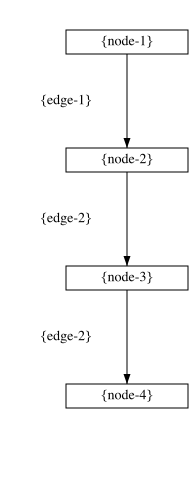
\includegraphics[width=\textwidth, angle=0]{figures/straight.pdf}
      \end{minipage}%
      \begin{minipage}[b][][b]{0.49\textwidth}
        \centering
        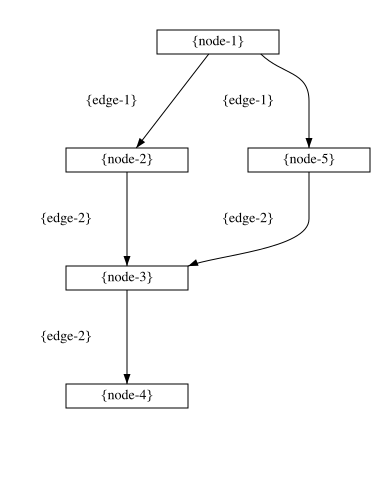
\includegraphics[width=\textwidth, angle=0]{figures/bifurcated.pdf}
      \end{minipage}%
      \captionsetup{type=figure}
      \caption{Graphs of tests}\label{graph_paige_tarjan_3}
    \end{minipage}\vspace{1em}

    The behavior of the two systems is the same by ignoring the labels on the edges and by considering them, so they are always bisimilar, so the test should not panic.

    The graphs have been generated using ReactionSystemsGUI using the nodes displayed in figure\ \ref{generating_graphs}. Note that to differentiate the two edges exiting \(\texttt{node-1}\) additional entities \(\texttt{left}\) and \(\texttt{right}\) are used, but are not displayed because the function for displaying the edges masks only for \(\texttt{edge-1}\) and \(\texttt{edge-2}\).

    \begin{minipage}{\textwidth}
      \centering
      \begin{minipage}{0.8\textwidth}
        \centering
        \includegraphics[width=\textwidth]{figures/straight_gui.png}
      \end{minipage}%

      \begin{minipage}{0.8\textwidth}
        \centering
        \includegraphics[width=\textwidth]{figures/bifurcated_gui.png}
      \end{minipage}%
      \captionsetup{type=figure}
      \caption{Generating graphs using ReactionSystemsGUI}\label{generating_graphs}
    \end{minipage}\vspace{1em}

    In addition to automated tests, some example inputs are provided in the folder \href{https://github.com/elvisrossi/ReactionSystems/tree/master/testing}{{\tt testing}}. The extension \(\texttt{.system}\) symbolizes system and associated instructions; the extension \(\texttt{.experiment}\) symbolizes an experiment, see\ \ref{experiment}.

    These examples were also used to do manual integration testing.

    The example \(\texttt{target.system}\)
    \begin{figure}[!ht]
      \centering
\begin{minted}{Text}
Environment: [x = {a}.y, y =({a}.{a, b}.nill + {b}.nill) ]
Initial Entities: {a, b}
Context: [({a,b}.{a}.{a,c}.x + {a,b}.{a}.{a}.nill)]
Reactions: ([{a,b}, {c}, {b}])

Target > Print,
Target (Limit: 7) > Print,
Target (Limit: 6) > Print,
Target (Limit: 5) > Print
\end{minted}
      \phantomsubcaption\label{example_target_system_instructions}
    \end{figure}
    generates as output:

\begin{minted}{Text}
After 6 steps we arrive at state:
{b}
After 6 steps we arrive at state:
{b}
After 6 steps we arrive at state:
{b}
After 5 steps we arrive at state:
{}
\end{minted}

    The output is correct since, as we can see from the graph of the system in figure\ \ref{graph_target_system} that the system has as leftmost production six states and the end state has entities set \(\texttt{\{b\}}\).

    \begin{figure}[h]
      \centering
      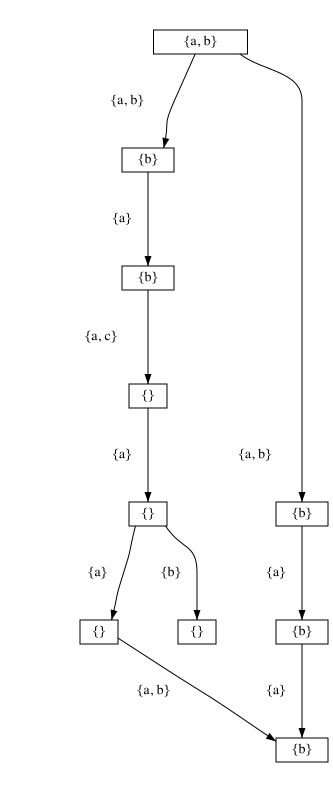
\includegraphics[width=0.5\textwidth, height=0.46\textheight, keepaspectratio]{figures/target_system.pdf}
      \caption{Graph of example\ \ref{example_target_system_instructions}, nodes have available entities as label, edges have the entities provided by the context as labels.}\label{graph_target_system}
    \end{figure}

    A small Perl script is provided that can convert systems created for the Prolog version of the program into the syntax described in\ \ref{design_system}. The script was used to convert systems that model mutual exclusion (MEX) available in the folder \href{https://github.com/elvisrossi/ReactionSystems/tree/master/testing/mex}{\(\texttt{testing/mex}\)}.

    A MEX system is composed of \(n\) looping processes, which only one can be in the critical section. Each process is identified by \(\texttt{out\_i}\) if is out of the critical section, \(\texttt{req\_i}\) if has requested to enter the critical section and \(\texttt{in\_i}\) if is in the critical section. Without the token \(\texttt{act\_i}\) no process can change state:

\begin{minted}{Text}
[{out_1}, {act_1}, {out_1}];
[{req_1}, {act_1}, {req_1}];
[{in_1}, {act_1}, {in_1}];
\end{minted}

    And \(\texttt{act\_i}\) is required to change state:

\begin{minted}{Text}
[{out_1, act_1}, {}, {req_1}];
\end{minted}

    Any subset of processes can be activated, the requests are preserved:

\begin{minted}{Text}
[{req_1, act_1, act_2}, {}, {req_1}];
[{req_1, act_1, act_3}, {}, {req_1}];
...
[{req_1, act_1, act_n}, {}, {req_1}];
\end{minted}

    Entering the critical section is handled by two other entities: \(\texttt{lock}\), which symbolizes that a process is in the critical section, and \(\texttt{done}\), which symbolizes that the critical section has been exited. \(\texttt{lock}\) remains until done:

\begin{minted}{Text}
[{lock}, {done}, {lock}];
\end{minted}

    No other processes have to have the lock for a process to enter the critical section:

\begin{minted}{Text}
[{req_1,act_1},{lock,act_2,...,act_n},{in_1,lock}];
\end{minted}

    The execution of these examples is more computationally expensive with increasing \(n\). The execution of \(\texttt{mex10.system}\) took 78791.202 milliseconds to run the instruction\ \ref{instruction_mex} which generate the graph of the system, converts it to dot format and saves it.\vspace{1em}

    \begin{minipage}{\textwidth}
\begin{minted}{Text}
Digraph > Dot
	| Entities
	| Context
	| ! "white"
	| ! "black"
	> Save("out.dot")
\end{minted}
      \captionsetup{type=table, name=\textbf{Instruction}}
      \caption{Instruction for MEX systems.}\label{instruction_mex}
    \end{minipage}\vspace{1em}

    \(\texttt{mex5.system}\) takes instead 109.148 milliseconds to run.

    Performance has been analyzed using perf\cite{manualperf_2025} and flamegraph\cite{Ochtman2025}.

    \begin{figure}
      \centering
      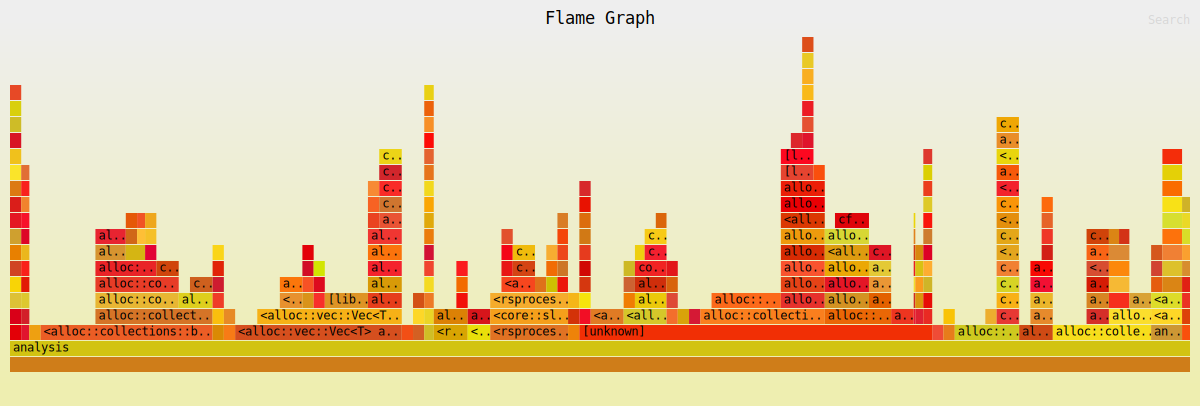
\includegraphics[width=\textwidth, height=0.5\textheight, keepaspectratio]{figures/flamegraph_mex5.pdf}
      \caption{Flamegraph of MEX RS with 5 processes.}
    \end{figure}

    \begin{figure}
      \centering
      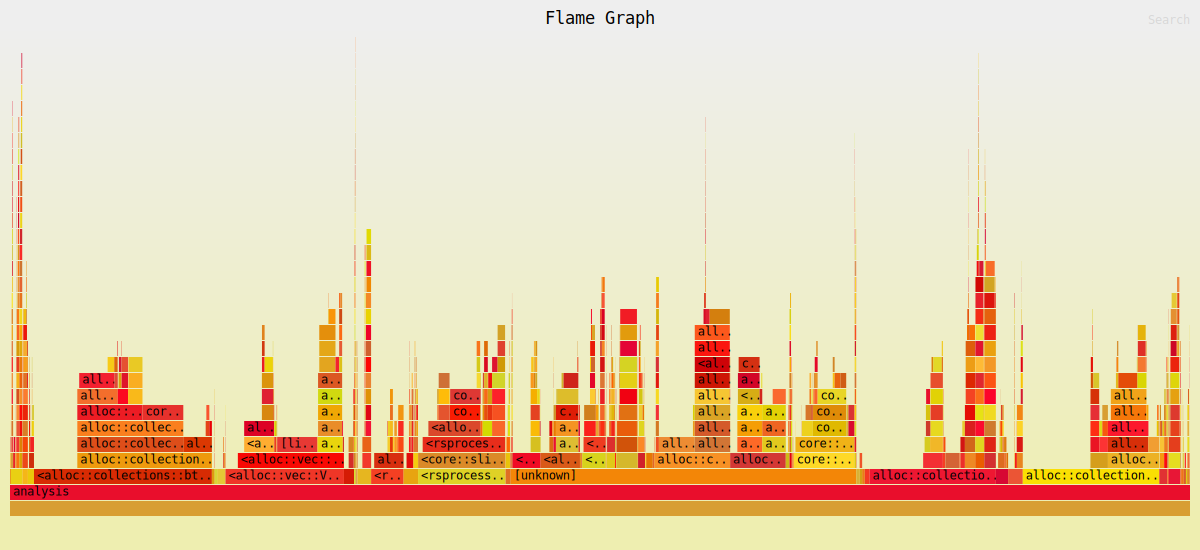
\includegraphics[width=\textwidth, height=0.5\textheight, keepaspectratio]{figures/flamegraph_mex10.pdf}
      \caption{Flamegraph of MEX RS with 10 processes.}
    \end{figure}

    Both of the flamegraphs share distinct features, but the one regarding MEX RS with 10 processes has finer resolution since the execution time is much longer. In decreasing order, some of the  that took most samples are:

    \begin{itemize}
    \item \(\texttt{unknown}\) that took 29\% of samples,
    \item \(\texttt{alloc::collections::btree::map::IntoIter::dying\_next}\) that took 14\% of samples,
    \item \(\texttt{<alloc::collections::btree::map::Iter as}\\\texttt{ core::iter::traits::iterator::Iterator>::next}\) that took 11\% of samples,
    \item \(\texttt{alloc::collections::btree::append::::bulk\_push}\) that took 11\% of samples,
    \item \(\texttt{alloc::collections::btree::map::BTreeMap::bulk\_build\_from\_sorted\_iter}\) that took 5,1\% of samples,
    \item \(\ldots\)
    \end{itemize}

    From the perf data we can gather that parsing took less than 3\% of total time, and that \(\texttt{unknown}\) refers to the methods belonging to System (section\ \ref{development_system}). This behavior is expected since most of the computation is carried by the structure that generates the graph.
  \end{section}

  \begin{section}{Validation}
    During development key issues identified from previous projects where performance and usability. The biggest problem with Prolog software is exceeding the stack limit and thus running out of memory. This problem is completely solved by using Rust. Another problem was that of performance. On dot file generation a 2 to 7 times performance improvement is seen, depending on the model simulated.

    Usability has been taken into account both for an end user and for a programmer that intend to expand the system: grammar follows general rules largely compatible with previous projects; the grammar is decoupled from the internal representation and thus permits greater maintainability and expandability; the use of traits permits more modularity and the coexistence of multiple types of RS in the same project; domain specific languages allow more efficient and intuitive instruction specification; the graphical user interface presents instructions and methods over reaction systems in a more intuitive way that with just a command line interface; the node system allows greater modularity and for easy additions of new instructions; easy SVG generation reduce the time spent between different software and speeds up the end user's tasks; saving the state of the application allows for lower friction when switching between projects; the web GUI provides a platform agnostic interface for quick development.
    Thus the original goal to develop a more user-friendly and developer-friendly reaction system modeler has been met.
  \end{section}
\end{chapter}

\begin{chapter}{Conclusion}
  Reaction Systems were originally conceived as a theoretical framework to model biochemical processes in living cells. Applying RS theory to practical modeling tasks has been non-trivial. The behavior of a RS can exhibit complex dynamics due to the non-monotonic role of inhibitors. In practice the number of entities and reactions can be large, making manual reasoning unfeasible without proper automated support.

  This thesis contributes to bridging the gap between RS theory and practical use by providing a concrete software realization of the formalism. The software is available in the repositories ReactionSystems\cite{ReactionSystemsGit} and ReactionSystemsGUI\cite{ReactionSystemsGUIGit}.

  \begin{section}{Summary of Contributions}
    \begin{itemize}
    \item New RS Modeling Platform: This thesis introduced a new software platform for Reaction Systems modeling, analysis and design, implemented in the Rust programming language for high performance and reliability. The software provides both a command-line interface (CLI), native graphical user interface (GUI) and a web based one. This enables users to model RSs either through text-based commands or in an interactive visual environment.

    \item Comprehensive Feature Set: The tool supports a rich set of features: simulation of RS, bisimulation of RSs, trace slicing, graph generation with multiple output formats like Dot, GraphML and SVG, loop analysis, automated conversion between types of RS.\ These features collectively offer a comprehensive toolkit for analyzing RS behavior.

    \item Performance and Design: The implementation in Rust allows to maximize performance, ensure safety and permit compositionality of future expansions. This eliminates prior memory issues with implementations in Prolog and dramatically improves execution speed. For example generating state-graph visualizations (Dot graphs) is now up to 7 times faster than before. Beyond performance, the software’s architecture was designed for clarity and extensibility: the RS grammar is kept independent of internal data structures to simplify maintenance, and core components use Rust traits to support modular extension.
    \end{itemize}
  \end{section}

  Future work may extend current models by a more in-depth performance analysis and optimization; may extend the methods available in the GUI;\ may provide new Reaction Systems types, like Quantitative Reaction Systems\cite{Mitrana_Păun_Petre_Prelipcean_2025} or Multiset Reaction Systems\cite{Bottoni_Mitrana_Petre_2025}; may provide methods to convert different structures like boolean networks into RS;\ or may provide additional test coverage of the current code.

\end{chapter}

\begin{chapter}{Appendix}
  \begin{section}{Running the software}
    \begin{subsection}{Reaction Systems}
      The code is available at the repository\ \cite{ReactionSystemsGit}.
      To download the software the git\ \cite{git} utility is recommended.

      To run the CLI a rust installation is necessary. It is recommended to install rustup\ \cite{rustup} from the official site or via a package manager:

\begin{minted}{Bash}
sudo apt install rustup

sudo dnf install rustup

sudo pacman -S rustup

brew install rustup
\end{minted}

      After installation run \mintinline{bash}{rustup default stable} to install a target.

      To build the code into an executable run \mintinline{bash}{cargo build --release}; to run the executable \mintinline{bash}{cargo run --release}.
      The repository contains only one executable workspace, called \(\texttt{analysis}\), that provides the CLI.\ It expects a path to a file with structure described in section\ \ref{instructions_analysis}.
    \end{subsection}

    \begin{subsection}{Reaction Systems GUI}
      The code is available at the repository\ \cite{ReactionSystemsGUIGit}.
      To download the software the git\ \cite{git} utility is recommended.

      To run the GUI a rust installation is necessary. It is recommended to install rustup\ \cite{rustup} from the official site or via a package manager:

\begin{minted}{Bash}
sudo apt install rustup

sudo dnf install rustup

sudo pacman -S rustup

brew install rustup
\end{minted}

      After installation run \mintinline{bash}{rustup default stable} to install a target. To install the wasm32 target a script is provided in the folder \(\texttt{reaction\_systems\_gui/}\) named \(\texttt{setup\_web.sh}\).

      A script is provided to check for errors during development in the folder \(\texttt{reaction\_systems\_gui/}\) called \(\texttt{check.sh}\).

      To format the code in a uniform way run \mintinline{bash}{cargo +nightly fmt}.

      To run the program use \mintinline{bash}{cargo run --release --features "persistence"}. % chktex 18
      The option \(\texttt{--features "persistence"}\)% chktex 18
      enables file reading and saving.

      To run the web application a script is provided in the folder \(\texttt{reaction\_systems\_gui/}\) called \(\texttt{build\_web.sh}\).
      The binary generated by rust is optimized using wasm-opt\ \cite{binaryen_2025}. It can be installed using a package manager:

\begin{minted}{bash}
sudo apt install binaryen

sudo dnf install binaryen

sudo pacman -S binaryen

brew install binaryen
\end{minted}

      The optimization step can be skipped by providing the flag \(\texttt{--fast}\) to the script.

      To run locally serve the files in the folder \(\texttt{reaction\_systems\_gui/docs/}\). This can be done with any simple http server. For example one can be installed by running \mintinline{bash}{cargo install basic-http-server}.
      A script is provided to run the server in the folder \(\texttt{reaction\_systems\_gui/}\) named \(\texttt{start\_server.sh}\).
    \end{subsection}
  \end{section}
\end{chapter}


\printbibliography%

\end{document}

%% - - - - - - - - - - - - - - - - - - - - - - - - - - - - - - - - - - - - - %%
